\chapter{THU THẬP, MÔ TẢ VÀ TỔNG QUAN CÁC BỘ DỮ LIỆU}

\startcontents[chapters]
\printmyminitoc{
Chương này trình bày nguồn gốc, cấu trúc, đặc điểm và mục đích sử dụng của các bộ dữ liệu trong báo cáo. Theo yêu cầu bài tập, nhóm dữ liệu được chia thành ba nhóm: dữ liệu dạng bảng, dữ liệu chuỗi thời gian/cảm biến và dữ liệu đa phương tiện.
}

\section{Tiêu chí lựa chọn dữ liệu}

Tiêu chí lựa chọn dữ liệu được xây dựng theo yêu cầu của đề bài và khả năng phân tích thực tế trong báo cáo. Mỗi bộ dữ liệu được đưa vào phải thuộc đúng một trong ba nhóm A, B hoặc C; có số mẫu và số biến đạt ngưỡng tối thiểu; có nguồn gốc rõ ràng; đồng thời có thể phục vụ các nội dung thống kê mô tả, trực quan hóa, tiền xử lý và học máy ở các chương sau.

Đối với nhóm A, dữ liệu phải là dạng bảng, có ít nhất hơn 5 thuộc tính và hơn 100 quan sát để phù hợp với phân tích biến định tính, biến định lượng và bài toán phân loại. Đối với nhóm B, dữ liệu phải có bản chất chuỗi thời gian hoặc tín hiệu/cảm biến, có hơn 500 quan sát để có thể biểu diễn xu hướng và đánh giá mô hình dự báo hoặc phân loại theo thời gian. Đối với nhóm C, dữ liệu phải thuộc nhóm đa phương tiện như ảnh hoặc văn bản, đủ lớn để trích xuất đặc trưng số và phân tích phân phối lớp.

Ngoài các tiêu chí định lượng, báo cáo ưu tiên những bộ dữ liệu có tài liệu mô tả, biến mục tiêu rõ ràng, đã được sử dụng trong nghiên cứu hoặc benchmark, và có khả năng tái lập bằng mã nguồn Python trong thư mục dự án. Nhờ vậy, việc lựa chọn dữ liệu không chỉ nhằm đáp ứng số lượng mà còn bảo đảm tính nhất quán giữa Chương 2, Chương 3 và Chương 4.

\section{Chiến lược thu thập và kiểm chứng dữ liệu}

Việc chọn dữ liệu trong báo cáo không chỉ nhằm đủ số lượng bộ dữ liệu theo đề bài, mà còn phải bảo đảm mỗi bộ dữ liệu có thể tạo ra phân tích thống kê, trực quan hóa và thí nghiệm học máy có ý nghĩa. Do đó, nhóm áp dụng bốn tiêu chí khi quyết định đưa một dataset vào báo cáo.

\begin{enumerate}
    \item \textbf{Tính phù hợp với nhóm dữ liệu}: dataset phải thuộc một trong ba nhóm A, B, C theo mô tả bài toán.
    \item \textbf{Khả năng phân tích thống kê}: dataset cần có biến định lượng hoặc biến định tính đủ rõ để tính thống kê, lập bảng tần suất và vẽ biểu đồ.
    \item \textbf{Khả năng học máy}: dataset nên có target hoặc có cấu trúc đặc trưng đủ tốt để phục vụ classification, regression hoặc clustering.
    \item \textbf{Khả năng tái lập}: dữ liệu, script, bảng kết quả, biểu đồ và log phải được lưu lại trong thư mục dự án.
\end{enumerate}

Với tiêu chí này, các bộ dữ liệu được chọn không đứng độc lập mà tạo thành một pipeline xuyên suốt. Heart Disease được dùng để minh họa lý thuyết, phân tích thống kê và classification. Appliances Energy được dùng để minh họa chuỗi thời gian và regression. HAM10000 và Reuters-21578 đại diện cho dữ liệu đa phương tiện, nơi dữ liệu thô cần được số hóa thành đặc trưng trước khi thống kê.

\begin{table}[H]
\centering
\caption{Vai trò của từng bộ dữ liệu trong toàn bộ báo cáo}
\label{tab:chapter2_dataset_role_matrix}
\small
\begin{tabular}{p{0.22\textwidth}p{0.18\textwidth}p{0.24\textwidth}p{0.24\textwidth}}
\toprule
Dataset & Nhóm & Vai trò thống kê & Vai trò học máy \\
\midrule
Heart Disease & A & Minh họa lý thuyết, outlier, tần suất & Classification, clustering \\
CDC Diabetes & A & Tần suất biến sức khỏe/hành vi & Classification nguy cơ tiểu đường \\
Breast Cancer & A & Histogram, boxplot, heatmap & Classification khối u \\
Appliances Energy & B & Line chart, phân phối target & Regression/time-series forecasting \\
HAR & B & Phân phối activity, cảm biến & Activity classification, clustering \\
MHEALTH & B & Thống kê tín hiệu cảm biến & Activity classification, clustering \\
HAM10000 & C & Phân phối lớp, đặc trưng ảnh & Image classification, clustering \\
Reuters-21578 & C & Độ dài văn bản, tần suất topic & Text classification \\
\bottomrule
\end{tabular}
\end{table}

Bảng \ref{tab:chapter2_dataset_role_matrix} cho thấy mỗi dataset đều có một vai trò cụ thể, tránh tình trạng thu thập dữ liệu chỉ để đủ số lượng. Đây cũng là căn cứ để Chương 3 và Chương 4 mở rộng phân tích theo từng nhóm.


Yêu cầu bài tập đặt ra ba nhóm dữ liệu chính. Nhóm A là dữ liệu dạng bảng, cần tối thiểu 3 bộ, mỗi bộ có hơn 5 features và hơn 100 samples. Nhóm B là dữ liệu chuỗi thời gian, cần tối thiểu 3 bộ, mỗi bộ có hơn 500 samples. Nhóm C là dữ liệu đa phương tiện, cần ít nhất 2 bộ trong các loại ảnh, audio, video hoặc text.

Trong quá trình thực hiện, báo cáo chọn 8 bộ dữ liệu để bao phủ cả ba nhóm. Các bộ dữ liệu được ưu tiên vì có nguồn công khai, có số mẫu đủ lớn, có bài toán học máy rõ ràng và có khả năng sinh bảng/hình/log minh chứng bằng Python. Bảng \ref{tab:dataset_overview} tóm tắt danh sách dữ liệu đã thu thập.

\begin{table}[H]
\centering
\caption{Đối chiếu bộ dữ liệu với yêu cầu đề bài}
\label{tab:chapter2_requirement_compliance}
\small
\begin{tabular}{p{0.18\textwidth}p{0.18\textwidth}p{0.16\textwidth}p{0.20\textwidth}p{0.18\textwidth}}
\toprule
Nhóm yêu cầu & Dataset sử dụng & Ngưỡng đề bài & Minh chứng đáp ứng & Artifact trong dự án \\
\midrule
A -- tabular & Heart Disease & $>5$ feature, $>100$ mẫu & 13 feature, 303 mẫu & \texttt{datasets/heart+disease/} \\
A -- tabular & CDC Diabetes & $>5$ feature, $>100$ mẫu & 21 feature, 253680 mẫu & \texttt{datasets/uci\_891\_cdc\_diabetes\_health\_indicators/} \\
A -- tabular & Breast Cancer & $>5$ feature, $>100$ mẫu & 30 feature, 569 mẫu & \texttt{datasets/breast+cancer+wisconsin+diagnostic/} \\
B -- chuỗi/cảm biến & Appliances Energy & $>500$ mẫu & 19735 mẫu, có mốc thời gian & \texttt{datasets/appliances+energy+prediction/} \\
B -- chuỗi/cảm biến & HAR & $>500$ mẫu & 10299 mẫu cảm biến & \texttt{datasets/human+activity+recognition/} \\
B -- chuỗi/cảm biến & MHEALTH & $>500$ mẫu & 1215745 mẫu cảm biến & \texttt{datasets/mhealth+dataset/} \\
C -- ảnh & HAM10000 & $\geq 500$ ảnh & 10015 ảnh/metadata & \texttt{datasets/skin-cancer-mnist-ham10000/} \\
C -- văn bản & Reuters-21578 & $\geq 1000$ văn bản & 21578 văn bản & \texttt{datasets/reuters-21578/} \\
\bottomrule
\end{tabular}
\end{table}

Bảng \ref{tab:chapter2_requirement_compliance} cho thấy lựa chọn dữ liệu vượt ngưỡng tối thiểu của đề bài: nhóm A có đủ ba bộ bảng, nhóm B có đủ ba bộ chuỗi/thứ tự quan sát, nhóm C có hai dạng multimedia là ảnh và văn bản. Việc ghi rõ thư mục artifact giúp báo cáo có tính tái lập: người đọc có thể kiểm tra dữ liệu thô, script phân tích trong \texttt{src/}, bảng xuất trong \texttt{outputs/tables/} và hình xuất trong \texttt{outputs/figures/}.

\begin{table}[H]
\centering
\caption{Tổng hợp các bộ dữ liệu sử dụng trong báo cáo}
\label{tab:dataset_overview}
\small
\begin{tabular}{llllr}
\toprule
ID & Nhóm & Bộ dữ liệu & Bài toán chính & Số mẫu \\
\midrule
A1 & A & Heart Disease & Classification & 303 \\
A2 & A & CDC Diabetes Health Indicators & Classification & 253680 \\
A3 & A & Breast Cancer Wisconsin Diagnostic & Classification & 569 \\
B1 & B & Appliances Energy Prediction & Regression & 19735 \\
B2 & B & Human Activity Recognition & Classification & 10299 \\
B3 & B & MHEALTH & Classification & 1215745 \\
C1 & C & HAM10000 & Image classification & 10015 \\
C2 & C & Reuters-21578 & Text classification & 21578 \\
\bottomrule
\end{tabular}
\end{table}


\section{Nhóm A: Dữ liệu dạng bảng}

Nhóm A gồm ba bộ dữ liệu dạng bảng, mỗi dòng là một quan sát độc lập và mỗi cột là một thuộc tính có kiểu dữ liệu rõ ràng. Các bảng mô tả trong phần này tập trung vào: số lượng mẫu, kiểu dữ liệu của feature, ý nghĩa thực tế và kết quả baseline dùng làm mốc đối sánh cho Chương 4.

\begin{table}[H]
\centering
\caption{Tổng hợp yêu cầu mô tả dữ liệu bảng nhóm A}
\label{tab:group_a_rubric_summary}
\small
\begin{tabular}{lllll}
\toprule
Dataset & Số mẫu & Số feature & Target & Bài toán \\
\midrule
A1 Heart Disease & 303 & 13 + target & num & Classification/clustering \\
A2 CDC Diabetes & 253680 & 21 + target & Diabetes\_binary & Classification \\
A3 Breast Cancer & 569 & 30 + target & Diagnosis & Classification \\
\bottomrule
\end{tabular}
\end{table}

\subsection{A1 - Heart Disease}

\textbf{Nguồn gốc và cấu trúc dữ liệu.} Heart Disease là bộ dữ liệu y khoa từ UCI Machine Learning Repository. Thư mục local là \path{datasets/heart+disease/}. Bộ dữ liệu gốc gồm Cleveland, Hungarian, Switzerland và Long Beach VA; trong báo cáo dùng bản Cleveland processed với 303 mẫu và 14 thuộc tính. Biến mục tiêu là \texttt{num}, trong đó 0 biểu diễn không có bệnh tim và 1--4 biểu diễn các mức có bệnh.

\textbf{Trường dữ liệu và phân phối.} Các biến chính gồm thông tin nhân khẩu học, triệu chứng lâm sàng và kết quả xét nghiệm: \texttt{age}, \texttt{sex}, \texttt{cp}, \texttt{trestbps}, \texttt{chol}, \texttt{thalach}, \texttt{oldpeak}, \texttt{ca}, \texttt{thal} và \texttt{num}. Phân phối target gồm 164 mẫu lớp 0 (54.13\%), 55 mẫu lớp 1, 36 mẫu lớp 2, 35 mẫu lớp 3 và 13 mẫu lớp 4; khi quy về nhị phân, hai nhóm không bệnh/có bệnh khá cân bằng. Tuổi bệnh nhân có trung bình 54.44, trung vị 56 và trải từ 29 đến 77. Cholesterol có trung bình 246.69 và giá trị lớn nhất ban đầu 564, sau làm sạch được chặn còn 371 để giảm ảnh hưởng outlier. \texttt{thalach} có trung bình 149.61, phản ánh nhịp tim tối đa khi gắng sức; \texttt{oldpeak} có trung vị 0.8 và giá trị cực đại được giảm từ 6.2 xuống 4.0 sau xử lý. Dữ liệu có missing value ở \texttt{ca} và \texttt{thal}, nên đây là ví dụ phù hợp để minh họa điền khuyết, mã hóa biến phân loại và chuẩn hóa trước khi học máy.

\textbf{Tổng quan bài báo liên quan.} Detrano và cộng sự xây dựng mô hình xác suất hỗ trợ chẩn đoán bệnh mạch vành từ dữ liệu lâm sàng, nhấn mạnh khả năng dùng biến bệnh án thường quy để ước lượng nguy cơ \cite{Detrano1989HeartDisease}. Aha và Kibler dùng cùng nhóm dữ liệu để đánh giá instance-based learning; trọng tâm của bài báo là đo khoảng cách giữa các hồ sơ bệnh nhân và ra quyết định dựa trên các ca tương tự \cite{Aha1991InstanceBased}. Gennari và cộng sự khai thác hướng conceptual clustering/classification qua hệ thống CLASSIT, cho thấy dữ liệu nhỏ nhưng giàu ý nghĩa y khoa vẫn có thể dùng để tạo nhóm khái niệm có thể diễn giải \cite{Gennari1989CLASSIT}. Nhìn chung, các nghiên cứu đạt được kết quả quan trọng ở mức phương pháp: chứng minh Heart Disease là benchmark phù hợp cho mô hình tuyến tính, k-NN, cây quyết định và ensemble; đồng thời cho thấy tính diễn giải của đặc trưng lâm sàng là yếu tố quan trọng hơn mô hình quá phức tạp.

\begin{table}[H]
\centering
\caption{Các biến chính trong Heart Disease}
\label{tab:heart_feature_dictionary}
\small
\begin{tabular}{llll}
\toprule
Biến & Loại & Ý nghĩa & Vai trò \\
\midrule
age & Định lượng rời rạc & Tuổi bệnh nhân & Feature \\
sex & Định tính & Giới tính & Feature \\
cp & Định tính & Loại đau ngực & Feature \\
trestbps & Liên tục & Huyết áp nghỉ ngơi & Feature \\
chol & Liên tục & Cholesterol huyết thanh & Feature \\
thalach & Liên tục & Nhịp tim tối đa & Feature \\
oldpeak & Liên tục & ST depression & Feature \\
ca & Rời rạc & Số mạch máu chính & Feature \\
thal & Định tính & Trạng thái thalassemia & Feature \\
num & Định tính/thứ bậc & Chẩn đoán bệnh tim & Target \\
\bottomrule
\end{tabular}
\end{table}

\begin{table}[H]
\centering
\caption{Thống kê mô tả các thuộc tính chính của Heart Disease}
\label{tab:heart_descriptive_stats}
\small
\begin{tabular}{lllll}
\toprule
Thuộc tính & Loại & Trung bình & Độ phân tán & Ghi chú \\
\midrule
age & Rời rạc & 54.44 & std = 9.04 & Tuổi, 29--77 \\
chol & Liên tục & 246.69 & std = 51.78 & Outlier max 564 \\
thalach & Liên tục & 149.61 & std = 22.88 & Nhịp tim tối đa \\
oldpeak & Liên tục & 1.04 & std = 1.16 & Lệch phải \\
num & Thứ bậc & -- & IQR theo lớp & Target 0--4 \\
\bottomrule
\end{tabular}
\end{table}

\begin{figure}[H]
\centering
\begin{subfigure}{0.92\textwidth}
    \centering
    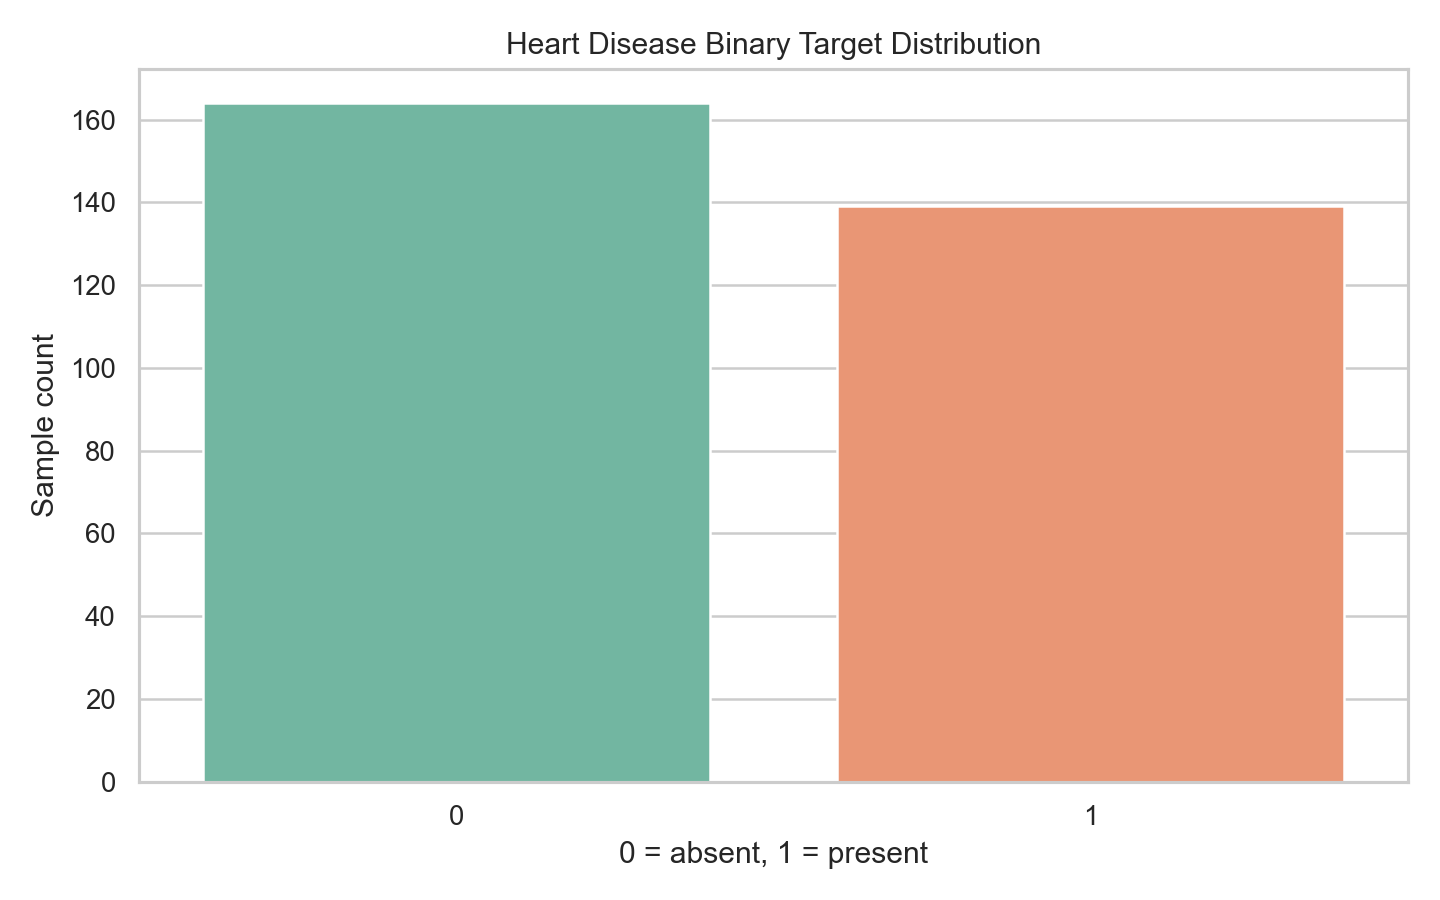
\includegraphics[width=\textwidth]{../outputs/figures/heart_disease_target_distribution.png}
    \caption{Phân phối target}
\end{subfigure}

\vspace{0.4cm}

\begin{subfigure}{0.92\textwidth}
    \centering
    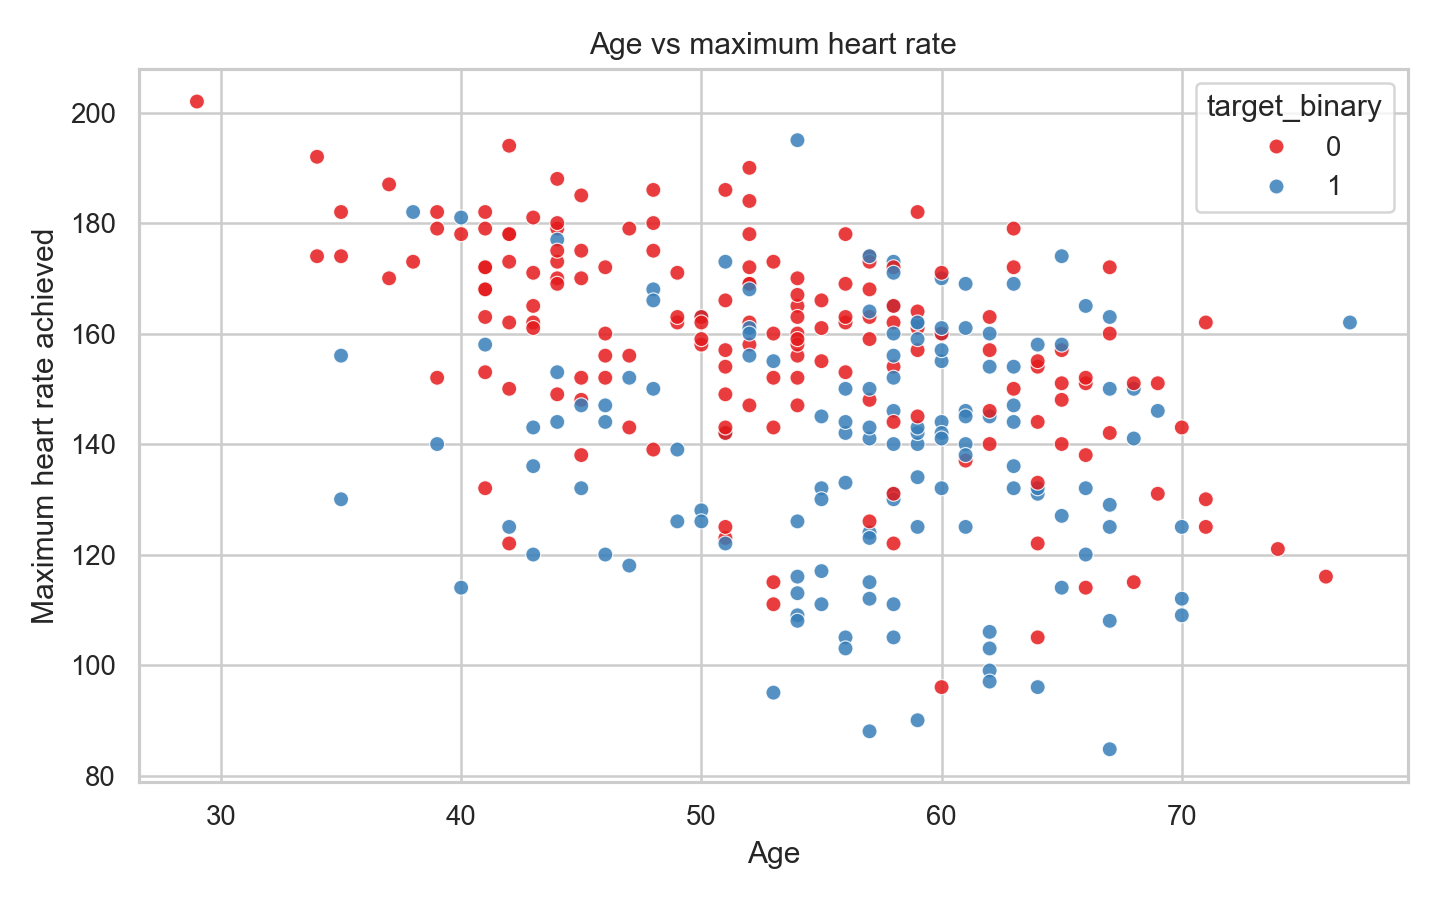
\includegraphics[width=\textwidth]{../outputs/figures/heart_disease_age_thalach_scatter.png}
    \caption{Tuổi và nhịp tim tối đa}
\end{subfigure}
\caption[Minh họa Heart Disease]{Minh họa Heart Disease. Python source: \texttt{src/analyze\_heart\_disease.py}; figure paths: \texttt{outputs/figures/heart\_disease\_target\_distribution.png}, \texttt{outputs/figures/heart\_disease\_age\_thalach\_scatter.png}.}
\label{fig:chapter2_heart_disease}
\end{figure}

\textbf{Kết quả ban đầu.} Bảng tần suất cho thấy target có hai nhóm chính sau khi quy về nhị phân: không bệnh và có bệnh. Baseline ở Bảng \ref{tab:chapter2_ml_preview} đạt F1 = 0.897 với Random Forest, cao hơn Logistic Regression và gần với SVM RBF. Hình \ref{fig:chapter2_heart_disease} minh họa mất cân bằng nhẹ của target và quan hệ giữa tuổi, \texttt{thalach} và nhãn bệnh.

\subsection{A2 - CDC Diabetes Health Indicators}

\textbf{Nguồn gốc và cấu trúc dữ liệu.} CDC Diabetes Health Indicators là bộ dữ liệu dạng bảng từ UCI, được lưu tại \path{datasets/uci_891_cdc_diabetes_health_indicators/}. Dữ liệu có 253,680 mẫu, 21 features và 1 target là \texttt{Diabetes\_binary}. Mỗi dòng biểu diễn một người trả lời khảo sát sức khỏe; các biến mô tả bệnh nền, hành vi sống, khả năng tiếp cận y tế, tự đánh giá sức khỏe và nhân khẩu học.

\textbf{Trường dữ liệu và phân phối.} Target \texttt{Diabetes\_binary} mất cân bằng rõ: 218,334 mẫu lớp 0 (86.07\%) và 35,346 mẫu lớp 1 (13.93\%). Nhóm bệnh nền gồm \texttt{HighBP}, \texttt{HighChol}, \texttt{Stroke}; nhóm hành vi gồm \texttt{Smoker}, \texttt{PhysActivity}, \texttt{Fruits}, \texttt{Veggies}; nhóm tự đánh giá gồm \texttt{GenHlth}, \texttt{MentHlth}, \texttt{PhysHlth}; nhóm xã hội học gồm \texttt{Sex}, \texttt{Age}, \texttt{Education}, \texttt{Income}. BMI có trung bình 28.38, trung vị 27 và khoảng giá trị thô 12--98; sau xử lý outlier, khoảng hợp lý hơn là 13.5--41.5. \texttt{MentHlth} và \texttt{PhysHlth} có trung vị 0 nhưng có giá trị cực đại 30 ngày, cho thấy phân phối lệch phải: phần lớn người trả lời không báo cáo ngày sức khỏe kém, nhưng một nhóm nhỏ có tình trạng kéo dài. \texttt{Age} có trung bình mã hóa 8.03, \texttt{Income} trung bình 6.05; đây là các biến ordinal nên không nên diễn giải như đại lượng liên tục tuyệt đối.

\textbf{Tổng quan bài báo liên quan.} Nguồn gốc dữ liệu gắn với hệ thống BRFSS của CDC, một khảo sát quy mô lớn về hành vi, bệnh nền và yếu tố nhân khẩu học trong cộng đồng \cite{CDC2023BRFSS}. Smith và cộng sự đóng gói bộ diabetes health indicators thành bài toán phân loại nguy cơ tiểu đường dựa trên dữ liệu tự báo cáo, giúp dữ liệu dễ dùng trong UCI/Kaggle và các thí nghiệm học máy \cite{Smith2014CDCIndicators}. Các nghiên cứu liên quan thường tóm tắt mục tiêu là phát hiện nhóm nguy cơ cao từ BMI, huyết áp, cholesterol, hoạt động thể chất, tuổi và thu nhập; kết quả đạt được là chứng minh dữ liệu khảo sát có thể dùng cho dự đoán sàng lọc, dù nhiễu do tự báo cáo và mất cân bằng lớp làm bài toán khó hơn dữ liệu y khoa đo trực tiếp. Điều này phù hợp với báo cáo hiện tại: mô hình đạt F1 trung bình khá, nhưng cần cân bằng lớp và đánh giá bằng recall/F1 thay vì chỉ accuracy.

\begin{table}[H]
\centering
\caption{Nhóm biến tiêu biểu trong CDC Diabetes}
\label{tab:cdc_feature_groups}
\small
\begin{tabular}{lll}
\toprule
Nhóm biến & Biến tiêu biểu & Ý nghĩa phân tích \\
\midrule
Bệnh nền & HighBP, HighChol, Stroke & Tình trạng sức khỏe nền \\
Hành vi & Smoker, PhysActivity, Fruits, Veggies & Lối sống và nguy cơ \\
Tiếp cận y tế & AnyHealthcare, NoDocbcCost & Khả năng chăm sóc sức khỏe \\
Tự đánh giá & GenHlth, MentHlth, PhysHlth & Sức khỏe tự báo cáo \\
Nhân khẩu & Sex, Age, Education, Income & Yếu tố xã hội học \\
\bottomrule
\end{tabular}
\end{table}

\begin{table}[H]
\centering
\caption{Thống kê mô tả các thuộc tính chính của CDC Diabetes}
\label{tab:cdc_descriptive_stats}
\small
\begin{tabular}{lllll}
\toprule
Thuộc tính & Loại & Trung bình & Độ phân tán & Ghi chú \\
\midrule
BMI & Liên tục & 28.38 & std = 6.61 & Lệch phải \\
GenHlth & Thứ bậc & 2.51 & std = 1.07 & Tự đánh giá sức khỏe \\
MentHlth & Rời rạc & 3.18 & std = 7.41 & Nhiều giá trị 0 \\
PhysHlth & Rời rạc & 4.24 & std = 8.72 & Nhiều giá trị 0 \\
Age & Thứ bậc & 8.03 & std = 3.05 & Mã nhóm tuổi \\
Income & Thứ bậc & 6.05 & std = 2.07 & Mã nhóm thu nhập \\
\bottomrule
\end{tabular}
\end{table}

\begin{figure}[H]
\centering
\begin{subfigure}{0.92\textwidth}
    \centering
    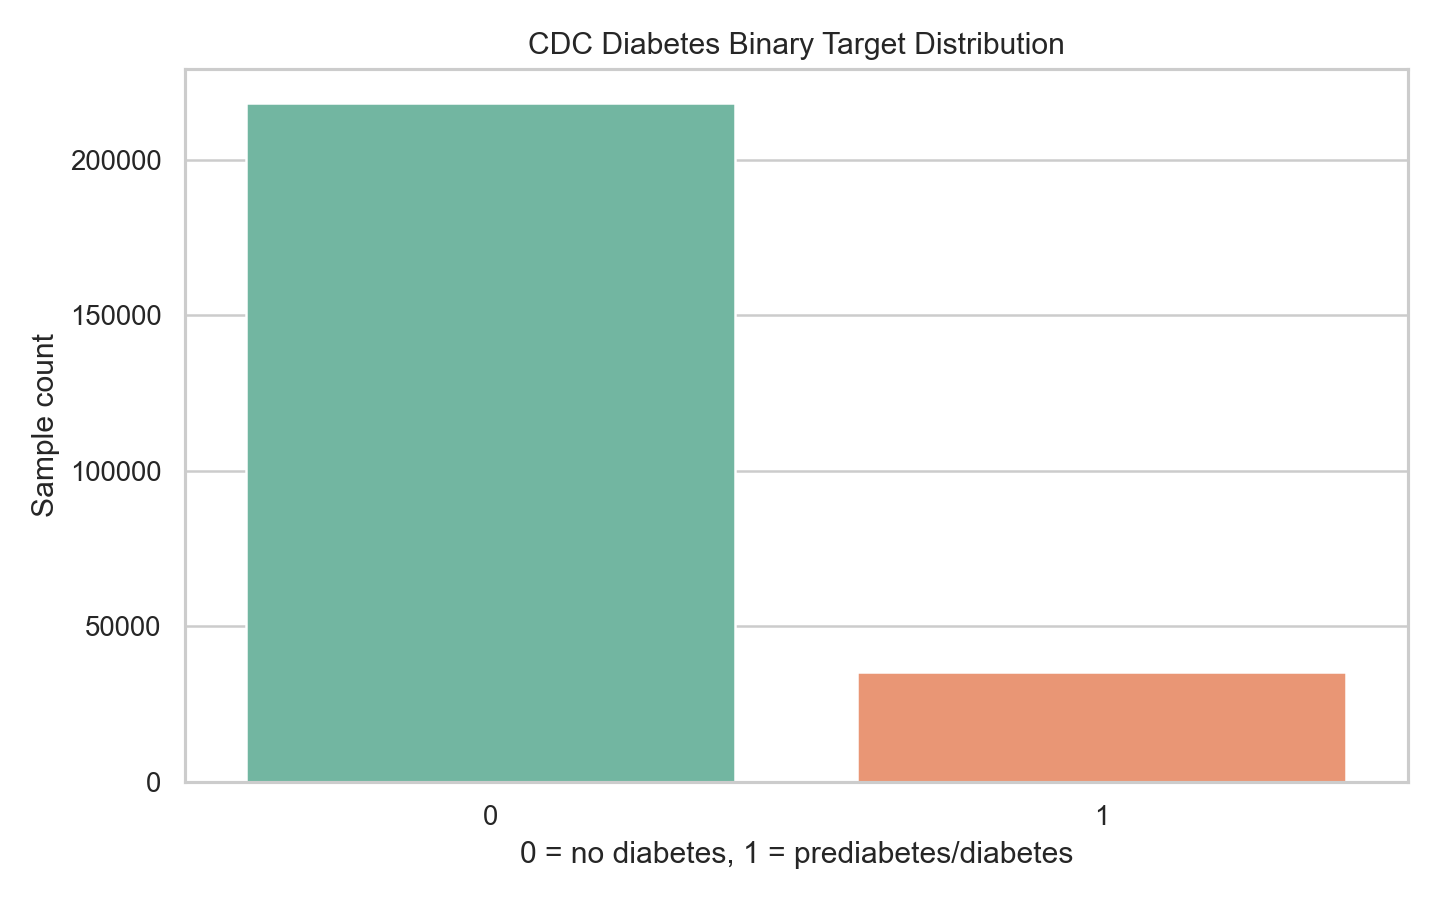
\includegraphics[width=\textwidth]{../outputs/figures/cdc_diabetes_target_distribution.png}
    \caption{Phân phối Diabetes\_binary}
\end{subfigure}

\vspace{0.4cm}

\begin{subfigure}{0.92\textwidth}
    \centering
    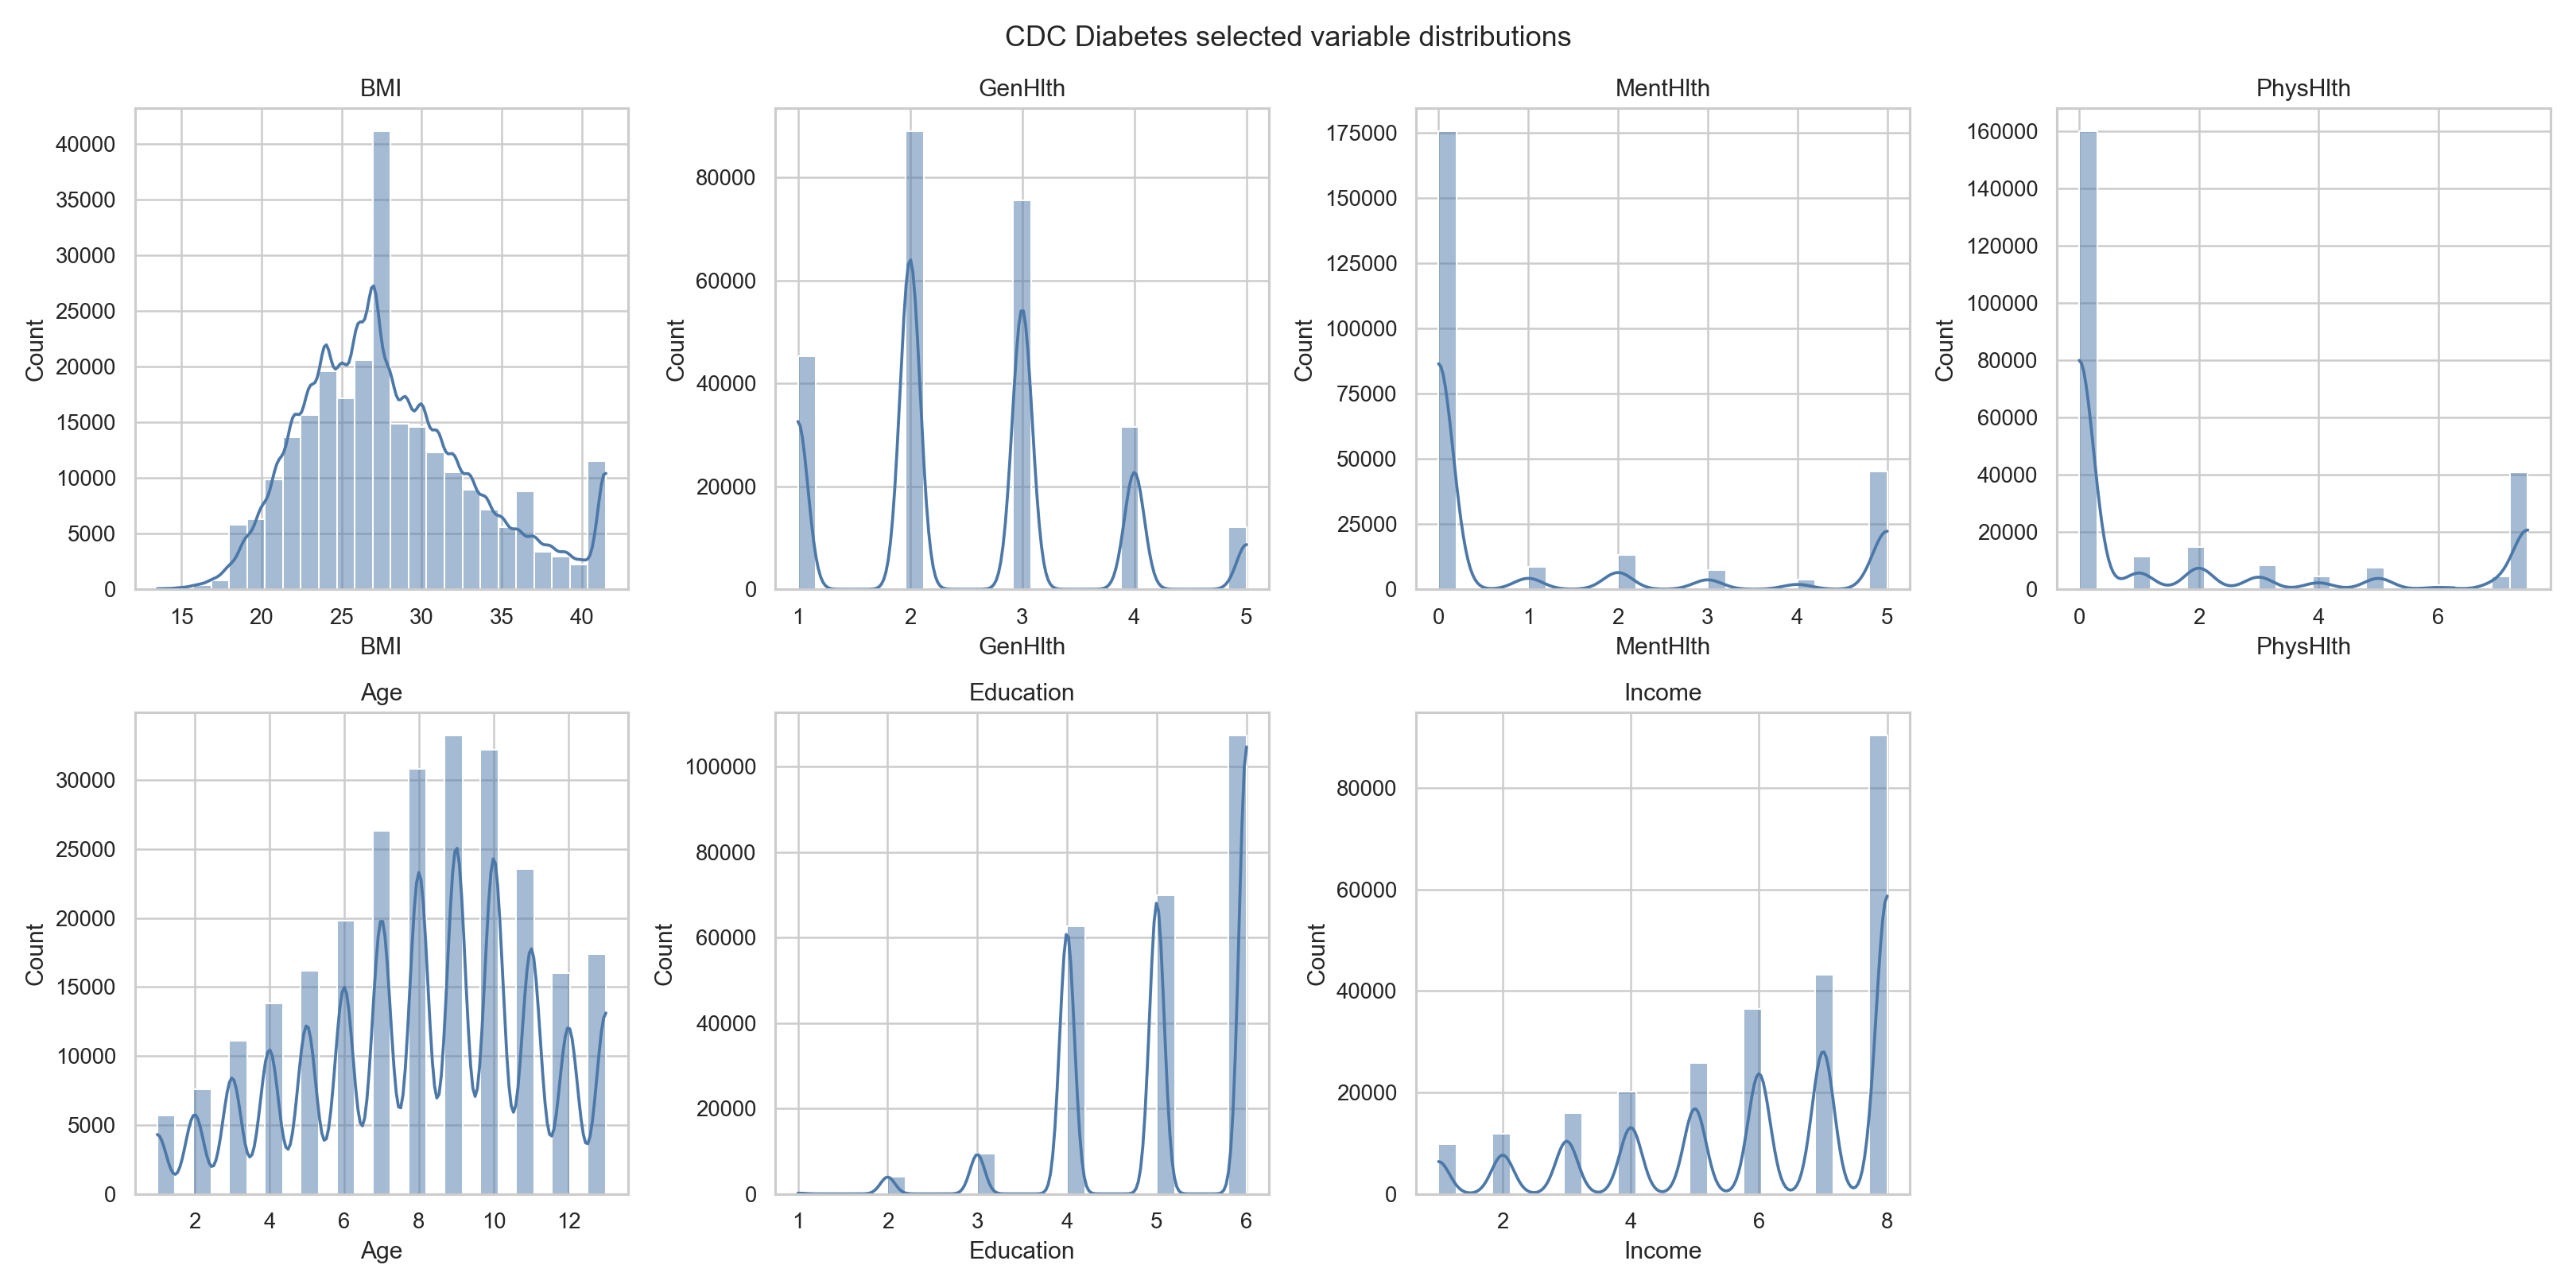
\includegraphics[width=\textwidth]{../outputs/figures/cdc_diabetes_selected_histograms.png}
    \caption{Histogram các biến sức khỏe}
\end{subfigure}
\caption[Minh họa CDC Diabetes]{Minh họa CDC Diabetes Health Indicators. Python source: \texttt{src/analyze\_cdc\_diabetes.py}; figure paths: \texttt{outputs/figures/cdc\_diabetes\_target\_distribution.png}, \texttt{outputs/figures/cdc\_diabetes\_selected\_histograms.png}. Bảng minh chứng bổ sung: \texttt{outputs/tables/cdc\_diabetes\_preprocessing\_comparison.csv}, \texttt{outputs/tables/cdc\_diabetes\_evidence\_index.csv}.}
\label{fig:chapter2_cdc_diabetes}
\end{figure}

\textbf{Kết quả ban đầu.} Dữ liệu có quy mô lớn nên phù hợp để kiểm tra ổn định của mô hình trên dữ liệu bảng nhiều biến ordinal/nhị phân. Baseline tốt nhất trong mẫu thử đạt F1 = 0.761 với SVM RBF, trong khi Logistic Regression đạt accuracy = 0.744. Hình \ref{fig:chapter2_cdc_diabetes} cho thấy target không cân bằng hoàn toàn và các biến như BMI, tuổi, sức khỏe tổng quát có phân phối lệch, cần chuẩn hóa hoặc biến đổi khi mô hình yêu cầu. Phân tích bổ sung theo mẫu Heart Disease được lưu trong \texttt{src/analyze\_cdc\_diabetes.py}; các bảng \texttt{cdc\_diabetes\_summary.csv}, \texttt{cdc\_diabetes\_preprocessing\_comparison.csv} và \texttt{cdc\_diabetes\_evidence\_index.csv} ghi lại đầy đủ thống kê mô tả, so sánh trước--sau xử lý và đường dẫn minh chứng.

\subsection{A3 - Breast Cancer Wisconsin Diagnostic}

\textbf{Nguồn gốc và cấu trúc dữ liệu.} Breast Cancer Wisconsin Diagnostic là bộ dữ liệu chẩn đoán ung thư vú từ UCI, được lưu tại \path{datasets/uci_17_breast_cancer_wisconsin_diagnostic/}. Bộ dữ liệu có 569 mẫu, 30 features và target \texttt{Diagnosis}. Target có hai lớp: malignant (M) và benign (B), tương ứng khối u ác tính và lành tính.

\textbf{Trường dữ liệu và phân phối.} Các features là đặc trưng hình học/kết cấu của nhân tế bào: radius, texture, perimeter, area, smoothness, compactness, concavity, concave points, symmetry và fractal dimension; mỗi nhóm có ba dạng mean, standard error và worst value. Phân phối lớp gồm 357 mẫu benign (62.74\%) và 212 mẫu malignant (37.26\%), không cân bằng hoàn toàn nhưng vẫn đủ mẫu cho cả hai lớp. \texttt{radius1} có trung bình 14.13 và trung vị 13.37; \texttt{area1} có trung bình 654.89, trung vị 551.1 và phương sai lớn, cho thấy kích thước khối u có outlier. Sau xử lý, \texttt{area1} được chặn từ max 2501 xuống 1326.3 và \texttt{radius1} từ 28.11 xuống 21.9. \texttt{concavity1} có trung vị 0.06154 nhưng max 0.4268, phản ánh độ lõm là biến phân biệt quan trọng giữa hai lớp. Heatmap cho thấy các biến radius, perimeter và area tương quan cao, vì vậy có thể cần chuẩn hóa và kiểm tra đa cộng tuyến trước khi dùng mô hình tuyến tính.

\textbf{Tổng quan bài báo liên quan.} Street, Wolberg và Mangasarian xây dựng bộ dữ liệu từ ảnh fine needle aspirate (FNA), sau đó trích xuất đặc trưng số mô tả nhân tế bào để chẩn đoán u lành/ác \cite{Street1993NuclearFeatures}. Điểm chính của bài báo là biến ảnh y sinh thành vector đặc trưng định lượng, giúp mô hình học máy có thể xử lý mà không cần ảnh gốc. Mangasarian và cộng sự tiếp tục khai thác hướng tối ưu hóa và separating hyperplane cho phân lớp ung thư vú \cite{Mangasarian1995BreastCancer}. Kết quả/ý nghĩa đạt được của các nghiên cứu này là chứng minh đặc trưng hình học của nhân tế bào có tính phân tách mạnh; trong báo cáo hiện tại, điều này được xác nhận khi SVM RBF đạt F1 = 0.976, cao nhất trong nhóm A.

\begin{table}[H]
\centering
\caption{Danh sách feature tiêu biểu của Breast Cancer}
\label{tab:breast_feature_dictionary}
\small
\begin{tabular}{llll}
\toprule
Nhóm feature & Loại & Ý nghĩa thực tế & Ví dụ \\
\midrule
radius/perimeter/area & Liên tục & Kích thước nhân tế bào & radius1, area1 \\
texture & Liên tục & Độ biến thiên cường độ ảnh & texture1 \\
smoothness/compactness & Liên tục & Hình dạng biên nhân & smoothness1 \\
concavity/concave points & Liên tục & Độ lõm và điểm lõm biên & concavity1 \\
symmetry/fractal dimension & Liên tục & Đối xứng và độ phức tạp biên & symmetry1 \\
Diagnosis & Định tính & Nhãn lành/ác tính & B, M \\
\bottomrule
\end{tabular}
\end{table}

\begin{table}[H]
\centering
\caption{Thống kê mô tả các thuộc tính chính của Breast Cancer}
\label{tab:breast_descriptive_stats}
\small
\begin{tabular}{lllll}
\toprule
Thuộc tính & Loại & Trung bình & Độ phân tán & Ghi chú \\
\midrule
radius1 & Liên tục & 14.13 & std = 3.52 & Kích thước nhân \\
texture1 & Liên tục & 19.29 & std = 4.30 & Kết cấu \\
area1 & Liên tục & 654.89 & std = 351.91 & Phân tán lớn \\
concavity1 & Liên tục & 0.09 & std = 0.08 & Biến phân biệt mạnh \\
Diagnosis & Định tính & -- & B/M = 357/212 & Target \\
\bottomrule
\end{tabular}
\end{table}

\begin{figure}[H]
\centering
\begin{subfigure}{0.92\textwidth}
    \centering
    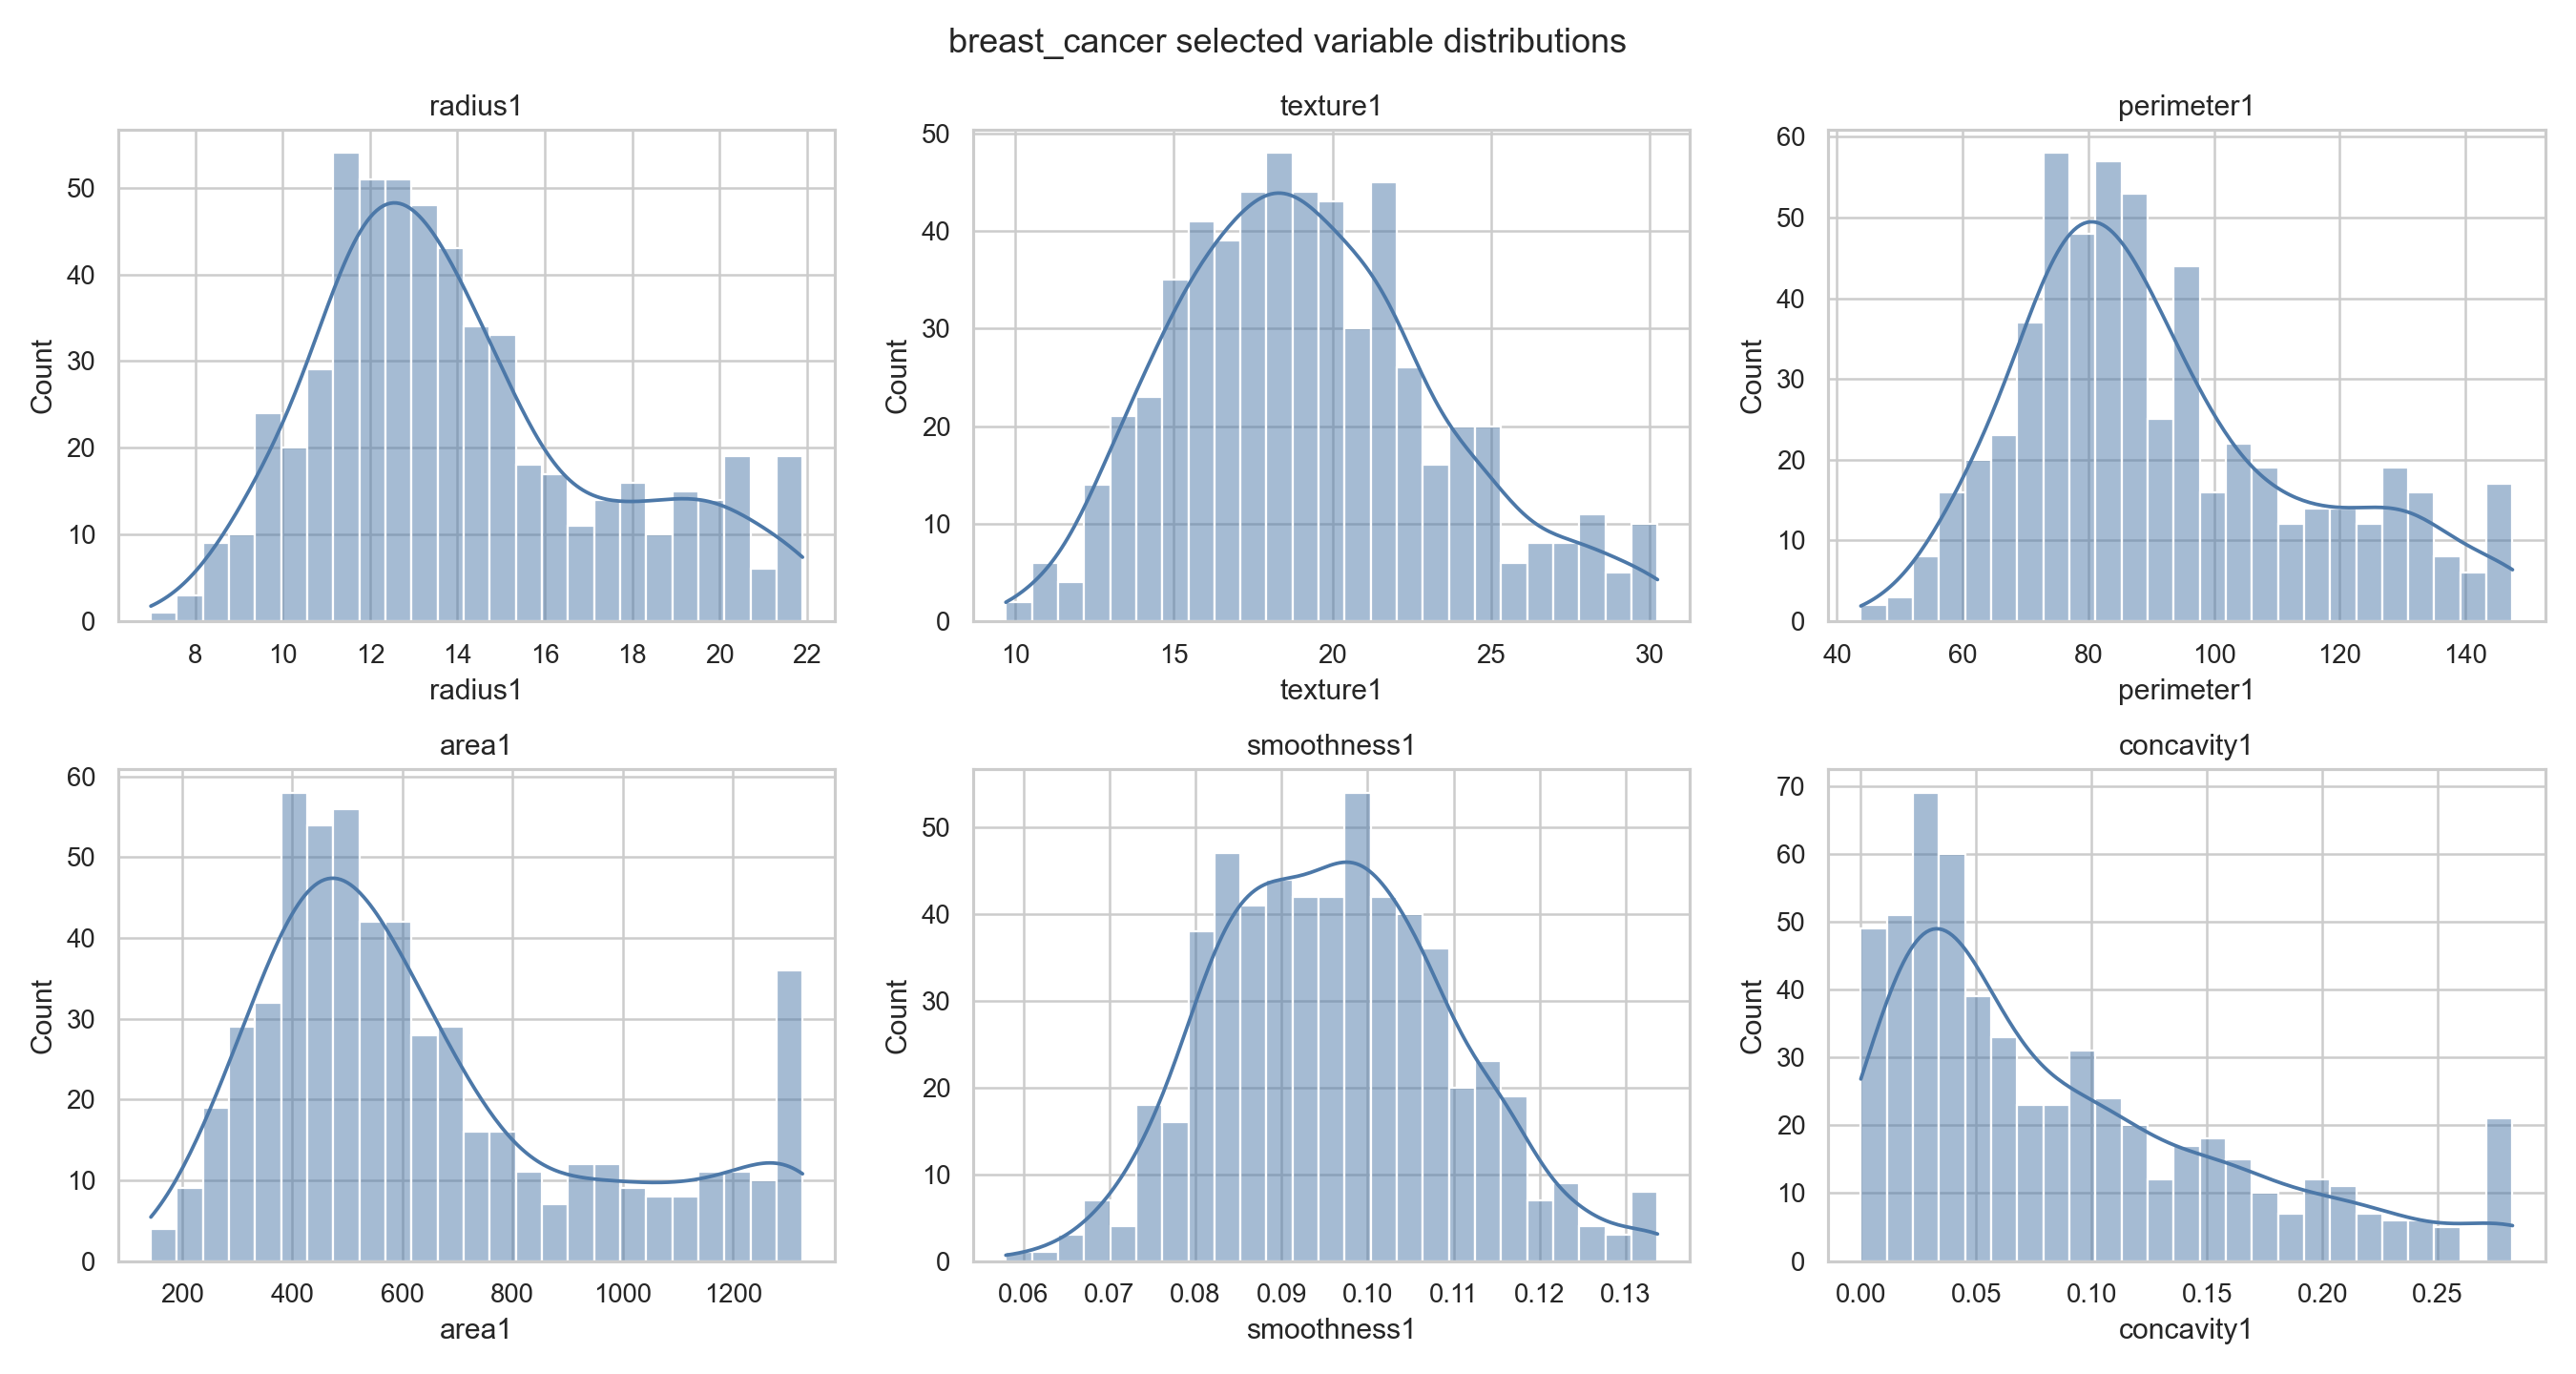
\includegraphics[width=\textwidth]{../outputs/figures/breast_cancer_selected_histograms.png}
    \caption{Histogram các biến chọn}
\end{subfigure}

\vspace{0.4cm}

\begin{subfigure}{0.92\textwidth}
    \centering
    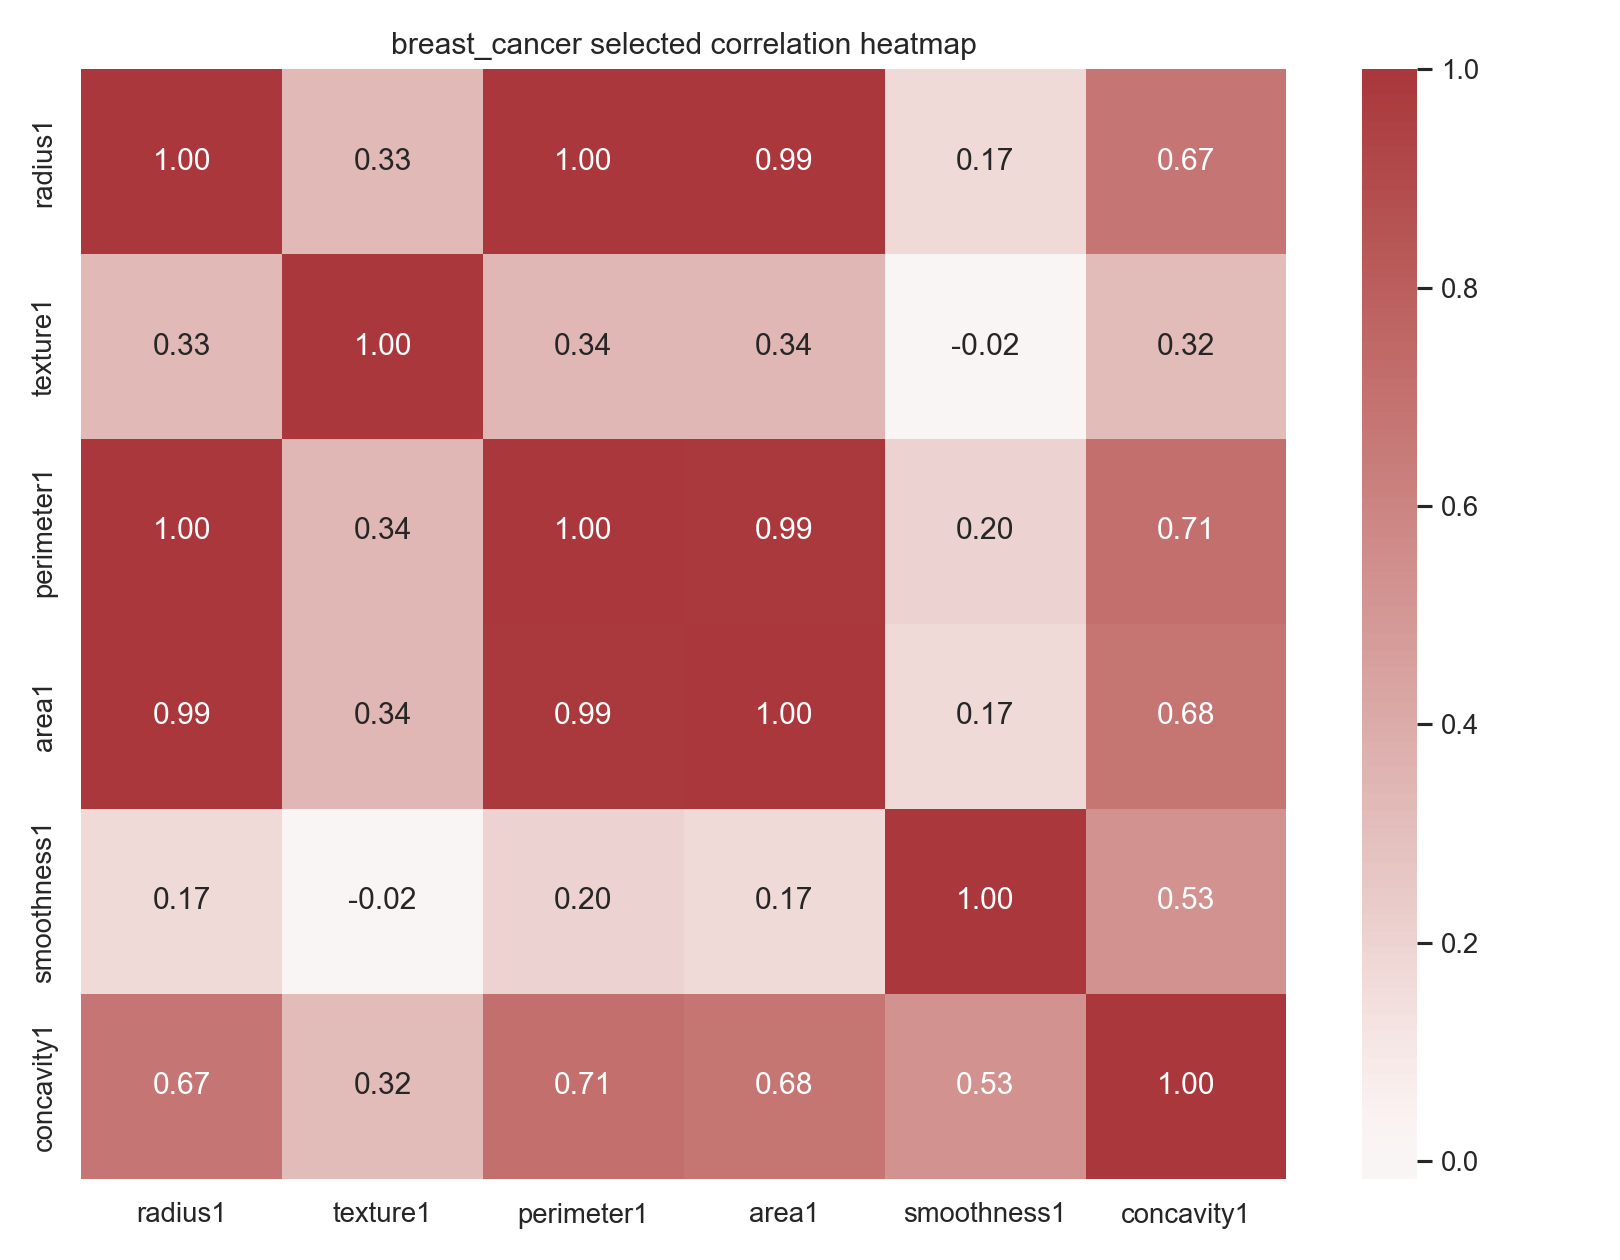
\includegraphics[width=\textwidth]{../outputs/figures/breast_cancer_correlation_heatmap.png}
    \caption{Heatmap tương quan}
\end{subfigure}
\caption[Minh họa cấu trúc số của Breast Cancer]{Minh họa cấu trúc số của Breast Cancer Wisconsin Diagnostic. Python source: \texttt{src/analyze\_tabular\_health.py}; figure paths: \texttt{outputs/figures/breast\_cancer\_selected\_histograms.png}, \texttt{outputs/figures/breast\_cancer\_correlation\_heatmap.png}.}
\label{fig:chapter2_breast_numeric}
\end{figure}

\textbf{Lý do chọn biểu đồ.} Histogram giúp xem hình dạng phân phối của các biến hình học; heatmap giúp phát hiện các nhóm biến tương quan cao trong Breast Cancer.

\textbf{Nhận xét.} Hình \ref{fig:chapter2_breast_numeric} cho thấy bộ Breast Cancer có nhiều biến liên tục và tương quan cao giữa các phép đo hình học. Điều này giải thích vì sao các mô hình tuyến tính sau chuẩn hóa, như Logistic Regression hoặc SVM, thường hoạt động tốt trên bộ dữ liệu này.

\textbf{Kết quả ban đầu.} Baseline SVM RBF đạt accuracy = 0.982 và F1 = 0.976, cao nhất trong ba bộ dữ liệu bảng nhóm A. Kết quả này phù hợp với nhận xét từ heatmap: nhiều đặc trưng hình học có khả năng phân tách rõ giữa malignant và benign.

\section{Nhóm B: Dữ liệu chuỗi thời gian và cảm biến}

Nhóm B gồm các bộ dữ liệu có yếu tố thứ tự thời gian hoặc tín hiệu cảm biến. Điểm khác biệt so với dữ liệu bảng là quan sát hiện tại có thể phụ thuộc vào thời điểm trước đó, nên cần mô tả tần suất thu thập, cửa sổ tín hiệu và cách tách train/test theo thời gian.

\begin{table}[H]
\centering
\caption{Tổng hợp đặc trưng chuỗi thời gian của nhóm B}
\label{tab:group_b_timeseries_summary}
\small
\begin{tabular}{p{0.18\textwidth}p{0.12\textwidth}p{0.14\textwidth}p{0.18\textwidth}p{0.24\textwidth}}
\toprule
Dataset & Số mẫu & Features & Tần suất/cửa sổ & Ý nghĩa chuỗi thời gian \\
\midrule
B1 Appliances & 19735 & 28 & 10 phút/mẫu & Dự báo tiêu thụ năng lượng theo thời gian \\
B2 HAR & 10299 & 561 & Cửa sổ tín hiệu inertial & Nhận dạng hoạt động từ chuỗi gia tốc/gyro \\
B3 MHEALTH & 1215745 & 23 & Log cảm biến liên tục & Chuyển log đa kênh thành cửa sổ hoạt động \\
\bottomrule
\end{tabular}
\end{table}

\subsection{B1 - Appliances Energy Prediction}

\textbf{Nguồn gốc và cấu trúc dữ liệu.} Appliances Energy Prediction là bộ dữ liệu UCI được lưu tại \path{datasets/uci_374_appliances_energy_prediction/}. Bộ dữ liệu có 19,735 mẫu, 28 features và target \texttt{Appliances}. Mỗi mẫu gắn với một mốc thời gian cách nhau khoảng 10 phút; khoảng quan sát bắt đầu từ 2016-01-11 17:00:00 đến 2016-05-27 18:00:00.

\textbf{Trường dữ liệu và phân phối.} Các features bao gồm nhiệt độ, độ ẩm trong nhiều khu vực, ánh sáng, áp suất, độ ẩm ngoài trời, tốc độ gió, tầm nhìn và điểm sương. Target \texttt{Appliances} có trung bình 97.69, trung vị 60, mode 50, độ lệch chuẩn 102.52 và hệ số biến thiên khoảng 1.05; max 1080 cho thấy phân phối lệch phải mạnh. Biến \texttt{lights} có trung vị và phân vị 75 đều bằng 0, nghĩa là phần lớn thời điểm đèn không tiêu thụ hoặc không được ghi nhận ở mức đáng kể. \texttt{T1} có trung bình 21.69, \texttt{RH\_1} trung bình 40.26 và \texttt{T\_out} trung bình 7.41, phản ánh đồng thời điều kiện trong nhà và ngoài trời. Vì đây là dữ liệu chuỗi thời gian, việc chia train/test phải theo thứ tự thời gian; nếu tách ngẫu nhiên sẽ làm rò rỉ thông tin tương lai và đánh giá mô hình quá lạc quan.

\textbf{Tổng quan bài báo liên quan.} Candanedo, Feldheim và Deramaix giới thiệu bộ dữ liệu này để dự báo tiêu thụ năng lượng thiết bị gia dụng từ cảm biến trong nhà và dữ liệu thời tiết \cite{Candanedo2017Appliances}. Bài báo gốc so sánh nhiều mô hình hồi quy, trong đó Random Forest đạt hiệu quả tốt nhờ mô hình hóa được quan hệ phi tuyến giữa nhiệt độ, độ ẩm, ánh sáng, điều kiện thời tiết và hành vi sử dụng thiết bị. Kết quả chính của nghiên cứu là chỉ ra dữ liệu cảm biến môi trường có thể dùng để dự báo năng lượng ở quy mô hộ gia đình, nhưng cần đặc trưng thời gian như giờ, ngày trong tuần, lag, rolling mean và rolling standard deviation. Trong báo cáo này, mô hình tuyến tính ban đầu có R2 thấp, xác nhận rằng nếu chưa tạo đặc trưng chuỗi thời gian thì mô hình khó khai thác đầy đủ mùa vụ và thói quen sinh hoạt.

\begin{table}[H]
\centering
\caption{Thống kê mô tả các thuộc tính chính của Appliances Energy}
\label{tab:appliances_descriptive_stats}
\small
\begin{tabular}{lllll}
\toprule
Thuộc tính & Loại & Trung bình & Độ phân tán & Ghi chú \\
\midrule
Appliances & Liên tục & 97.69 & std = 102.52 & Target lệch phải \\
lights & Liên tục & 3.80 & std = 7.94 & Nhiều giá trị 0 \\
T1 & Liên tục & 21.69 & std = 1.61 & Nhiệt độ trong nhà \\
RH\_1 & Liên tục & 40.26 & std = 3.98 & Độ ẩm trong nhà \\
T\_out & Liên tục & 7.41 & std = 5.32 & Nhiệt độ ngoài trời \\
Windspeed & Liên tục & 4.04 & std = 2.45 & Thời tiết \\
\bottomrule
\end{tabular}
\end{table}

\begin{figure}[H]
\centering
\begin{subfigure}{0.92\textwidth}
    \centering
    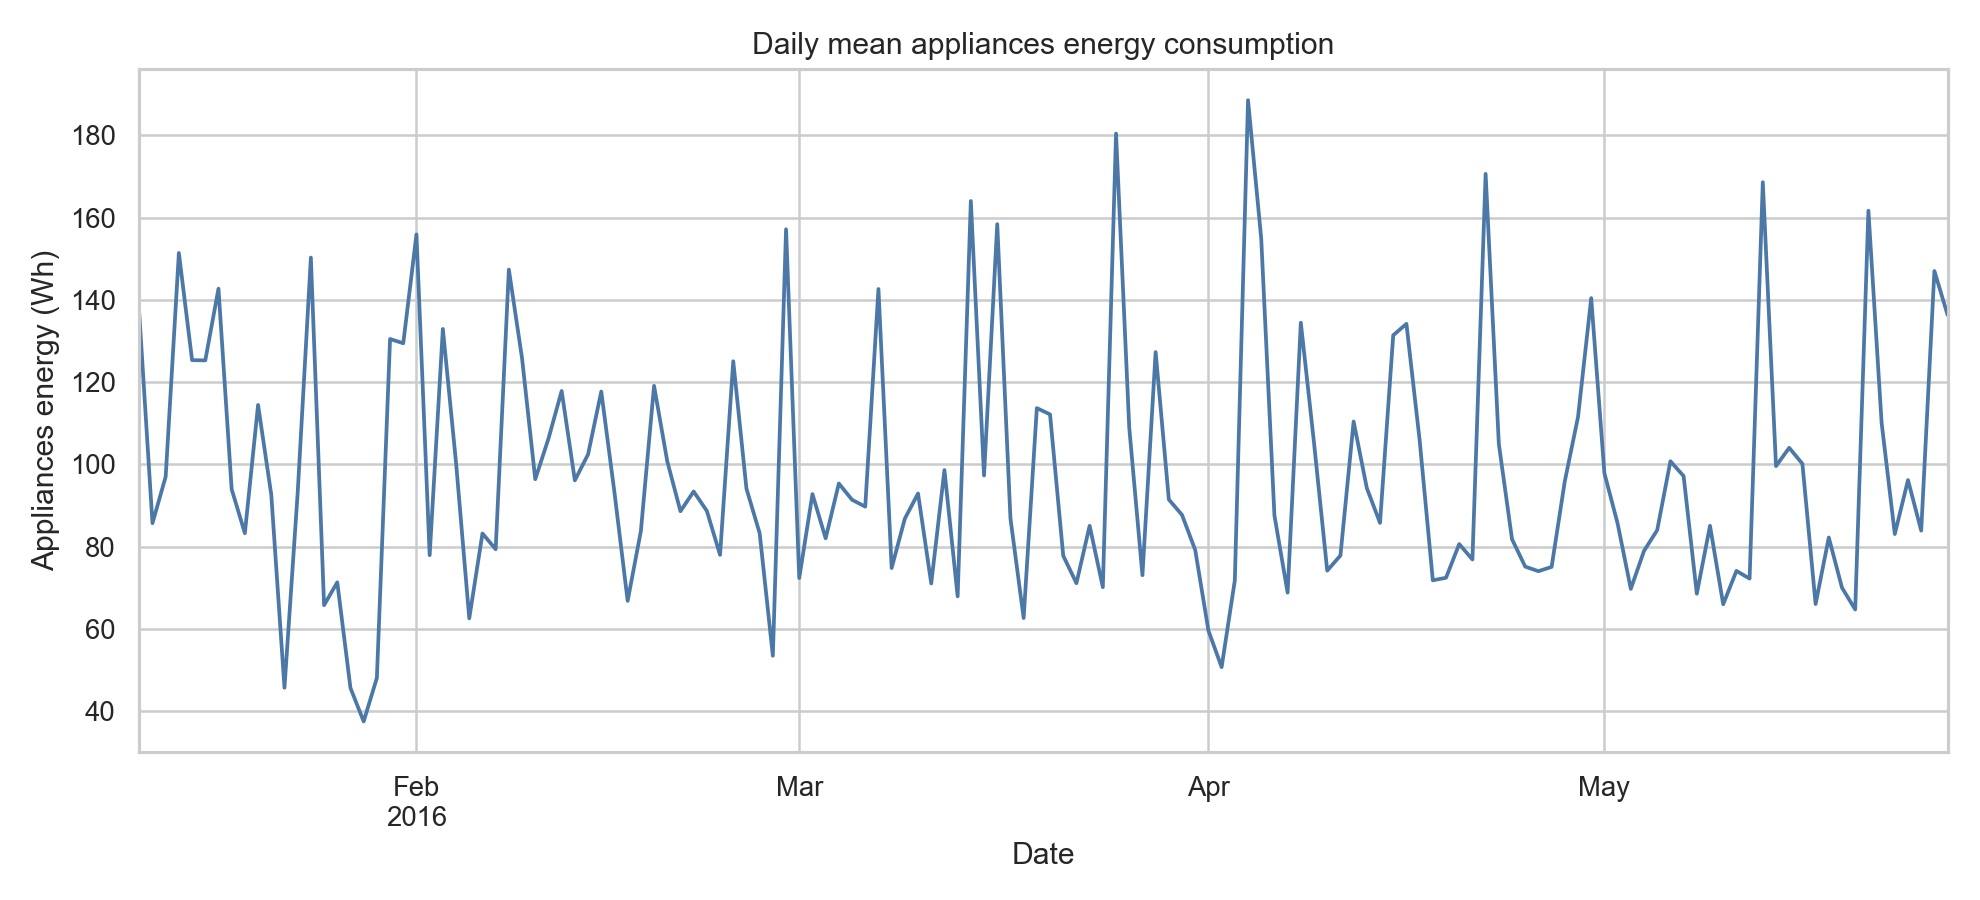
\includegraphics[width=\textwidth]{../outputs/figures/appliances_energy_daily_line.png}
    \caption{Tiêu thụ trung bình theo ngày}
\end{subfigure}

\vspace{0.4cm}

\begin{subfigure}{0.92\textwidth}
    \centering
    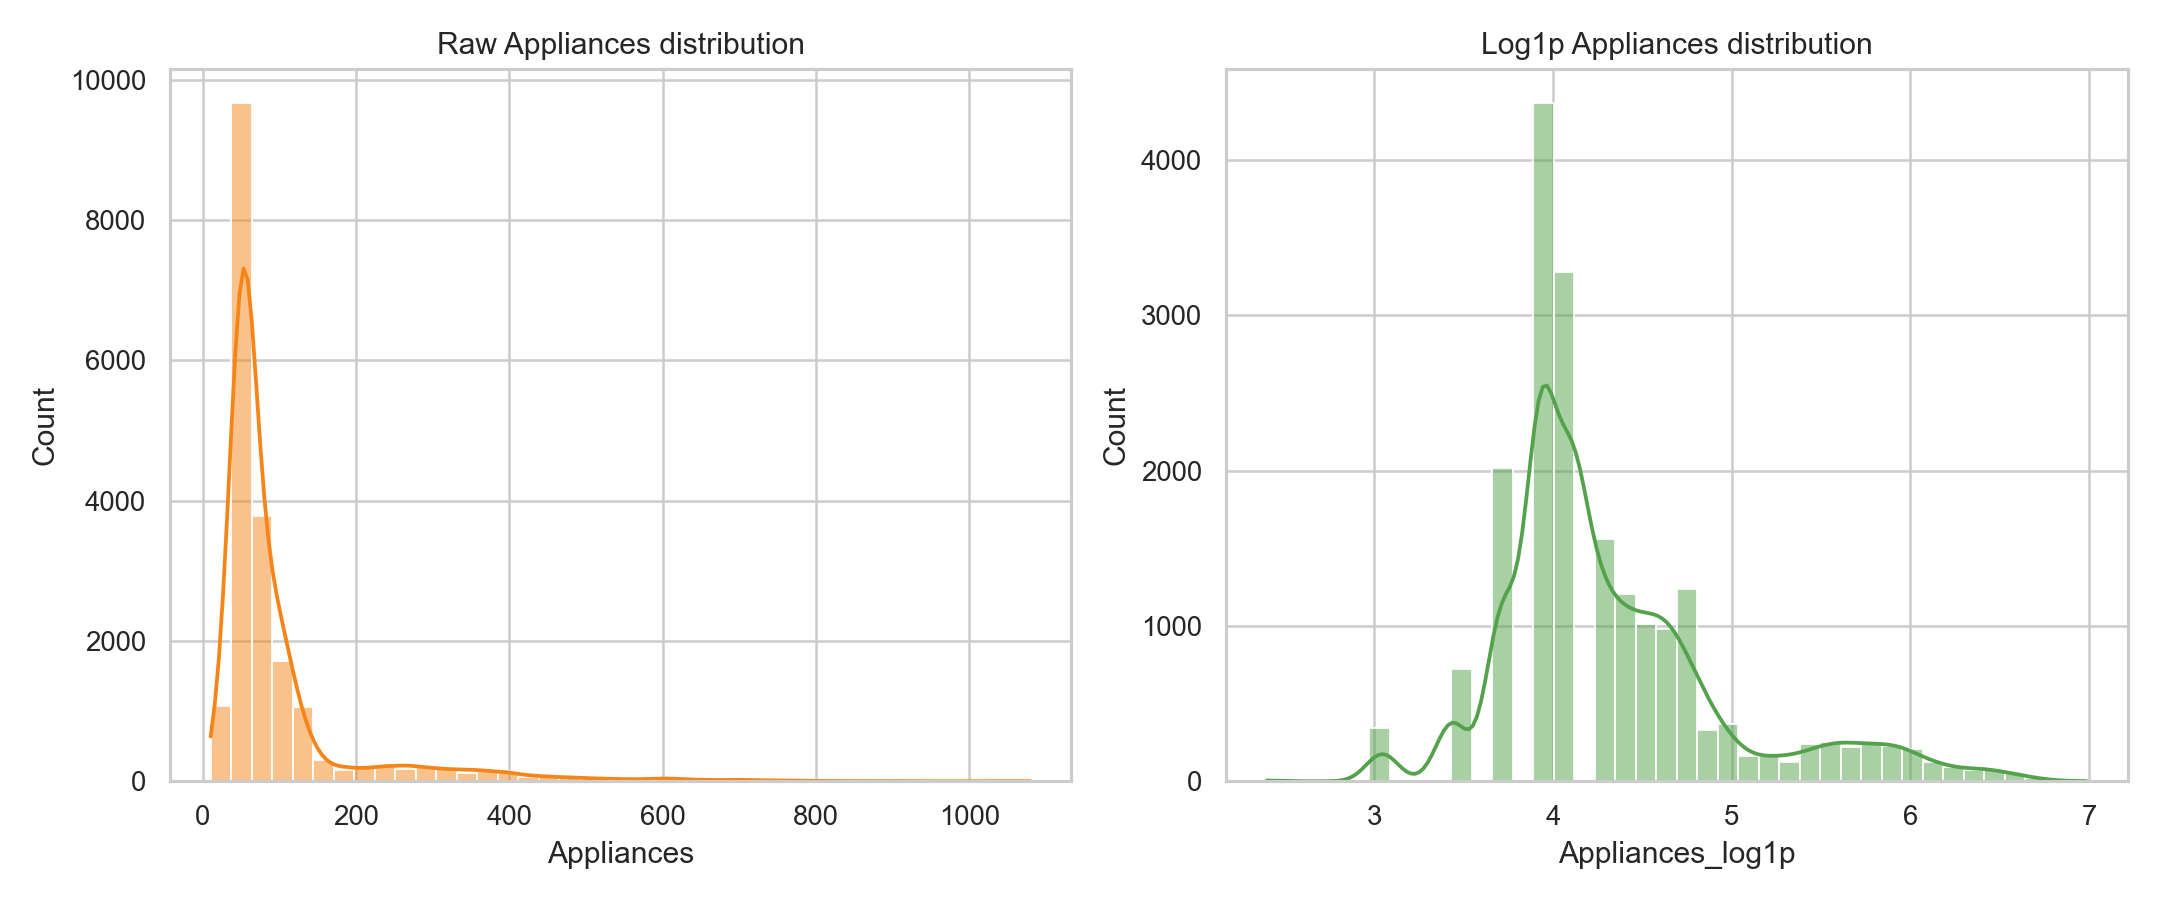
\includegraphics[width=\textwidth]{../outputs/figures/appliances_energy_distribution_raw_vs_log.png}
    \caption{Phân phối target trước/sau log}
\end{subfigure}
\caption[Minh họa đặc trưng chuỗi thời gian của Appliances Energy]{Minh họa đặc trưng chuỗi thời gian của Appliances Energy. Python source: \texttt{src/analyze\_appliances\_energy.py}; figure paths: \texttt{outputs/figures/appliances\_energy\_daily\_line.png}, \texttt{outputs/figures/appliances\_energy\_distribution\_raw\_vs\_log.png}.}
\label{fig:chapter2_appliances_timeseries}
\end{figure}

\textbf{Lý do chọn biểu đồ.} Line chart được chọn vì Appliances Energy là dữ liệu chuỗi thời gian; histogram raw-vs-log được chọn để kiểm tra mức lệch phải của target và tác dụng của log transform.

\textbf{Nhận xét.} Hình \ref{fig:chapter2_appliances_timeseries} cho thấy dữ liệu Appliances có biến động theo thời gian và phân phối target lệch phải. Do đó, ngoài các mô hình regression thông thường, các đặc trưng lag, rolling mean và log transform có thể cần thiết để cải thiện kết quả dự báo.

\textbf{Kết quả ban đầu.} Khi tách train/test theo thứ tự thời gian, Linear Regression đạt MAE = 58.71 và RMSE = 89.40. Random Forest chưa tốt trong cấu hình ban đầu vì chưa bổ sung đủ đặc trưng lag/rolling, cho thấy bài toán dự báo năng lượng cần xử lý seasonality và đặc trưng thời gian cẩn thận hơn classification dữ liệu bảng.

\subsection{B2 - Human Activity Recognition Using Smartphones}

\textbf{Nguồn gốc và cấu trúc dữ liệu.} Human Activity Recognition Using Smartphones (HAR) là bộ dữ liệu cảm biến chuyển động từ UCI, được giải nén tại \path{datasets/human+activity+recognition+using+smartphones/UCI HAR Dataset/}. Bộ dữ liệu có 10,299 mẫu, 561 features và 6 nhãn hoạt động: walking, walking upstairs, walking downstairs, sitting, standing và laying. Dữ liệu gồm feature vectors đã xử lý và tín hiệu inertial raw trong thư mục train/test.

\textbf{Trường dữ liệu và phân phối.} 561 features được trích từ accelerometer và gyroscope, bao gồm đặc trưng miền thời gian, miền tần số, trung bình, độ lệch chuẩn, năng lượng, entropy, tương quan giữa trục và dominant frequency. Phân phối lớp tương đối cân bằng: LAYING 1,944 mẫu (18.88\%), STANDING 1,906 (18.51\%), SITTING 1,777 (17.25\%), WALKING 1,722 (16.72\%), WALKING\_UPSTAIRS 1,544 (14.99\%) và WALKING\_DOWNSTAIRS 1,406 (13.65\%). Nhóm hoạt động tĩnh (sitting, standing, laying) và nhóm hoạt động động (walking, upstairs, downstairs) có mẫu dao động cảm biến khác nhau; đây là cơ sở để boxplot theo activity cho thấy khả năng phân tách trước khi huấn luyện mô hình.

\textbf{Tổng quan bài báo liên quan.} Anguita và cộng sự công bố HAR như benchmark nhận dạng hoạt động bằng smartphone, sử dụng cảm biến gia tốc và con quay hồi chuyển thu thập trên cửa sổ tín hiệu cố định \cite{Anguita2013HAR}. Bài báo tóm tắt quy trình từ tín hiệu raw, lọc nhiễu, trích xuất 561 đặc trưng rồi huấn luyện SVM để phân loại sáu hoạt động. Kết quả/ý nghĩa đạt được là chứng minh điện thoại thông minh có thể thay thế thiết bị chuyên dụng trong activity recognition, đồng thời cung cấp bộ feature vector chuẩn cho so sánh mô hình. Với báo cáo hiện tại, phân phối lớp khá cân bằng giúp classification/clustering đáng tin cậy hơn MHEALTH, còn tín hiệu raw mở ra hướng dùng CNN 1D hoặc LSTM nếu mở rộng sang học sâu.

\begin{table}[H]
\centering
\caption{Cấu trúc nhãn hoạt động trong HAR}
\label{tab:har_activity_labels}
\small
\begin{tabular}{ll}
\toprule
Mã nhãn & Hoạt động \\
\midrule
1 & WALKING \\
2 & WALKING\_UPSTAIRS \\
3 & WALKING\_DOWNSTAIRS \\
4 & SITTING \\
5 & STANDING \\
6 & LAYING \\
\bottomrule
\end{tabular}
\end{table}

\begin{table}[H]
\centering
\caption{Thống kê mô tả các thuộc tính chính của HAR}
\label{tab:har_descriptive_stats}
\small
\begin{tabular}{lllll}
\toprule
Thuộc tính & Loại & Trung bình & Độ phân tán & Ghi chú \\
\midrule
f001\_tBodyAcc-mean()-X & Liên tục & 0.27 & std = 0.07 & Gia tốc trục X \\
f004\_tBodyAcc-std()-X & Liên tục & -0.61 & std = 0.45 & Dao động tín hiệu \\
f121\_tBodyGyro-mean()-X & Liên tục & -0.03 & std = 0.13 & Gyro trục X \\
activity & Định tính & -- & 6 lớp & Target khá cân bằng \\
subject & Định tính & -- & 30 người & Nhóm quan sát \\
\bottomrule
\end{tabular}
\end{table}

\begin{figure}[H]
\centering
\begin{subfigure}{0.92\textwidth}
    \centering
    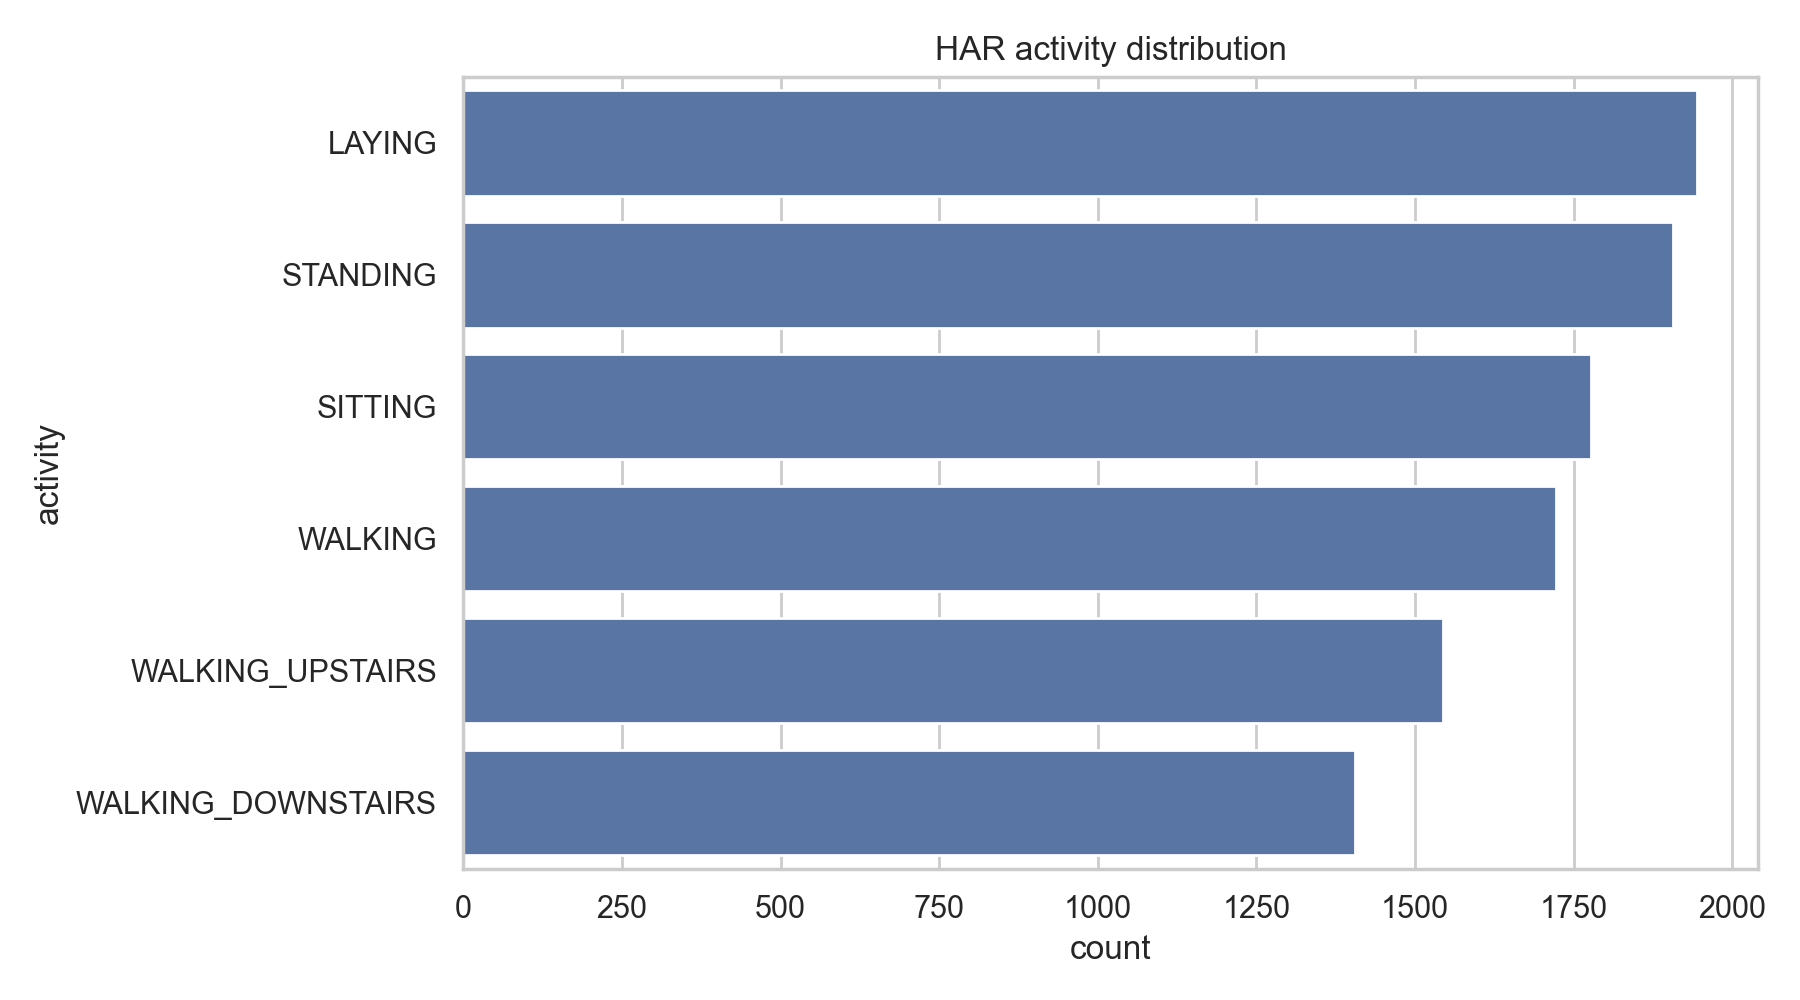
\includegraphics[width=\textwidth]{../outputs/figures/har_activity_distribution.png}
    \caption{Phân phối activity}
\end{subfigure}

\vspace{0.4cm}

\begin{subfigure}{0.92\textwidth}
    \centering
    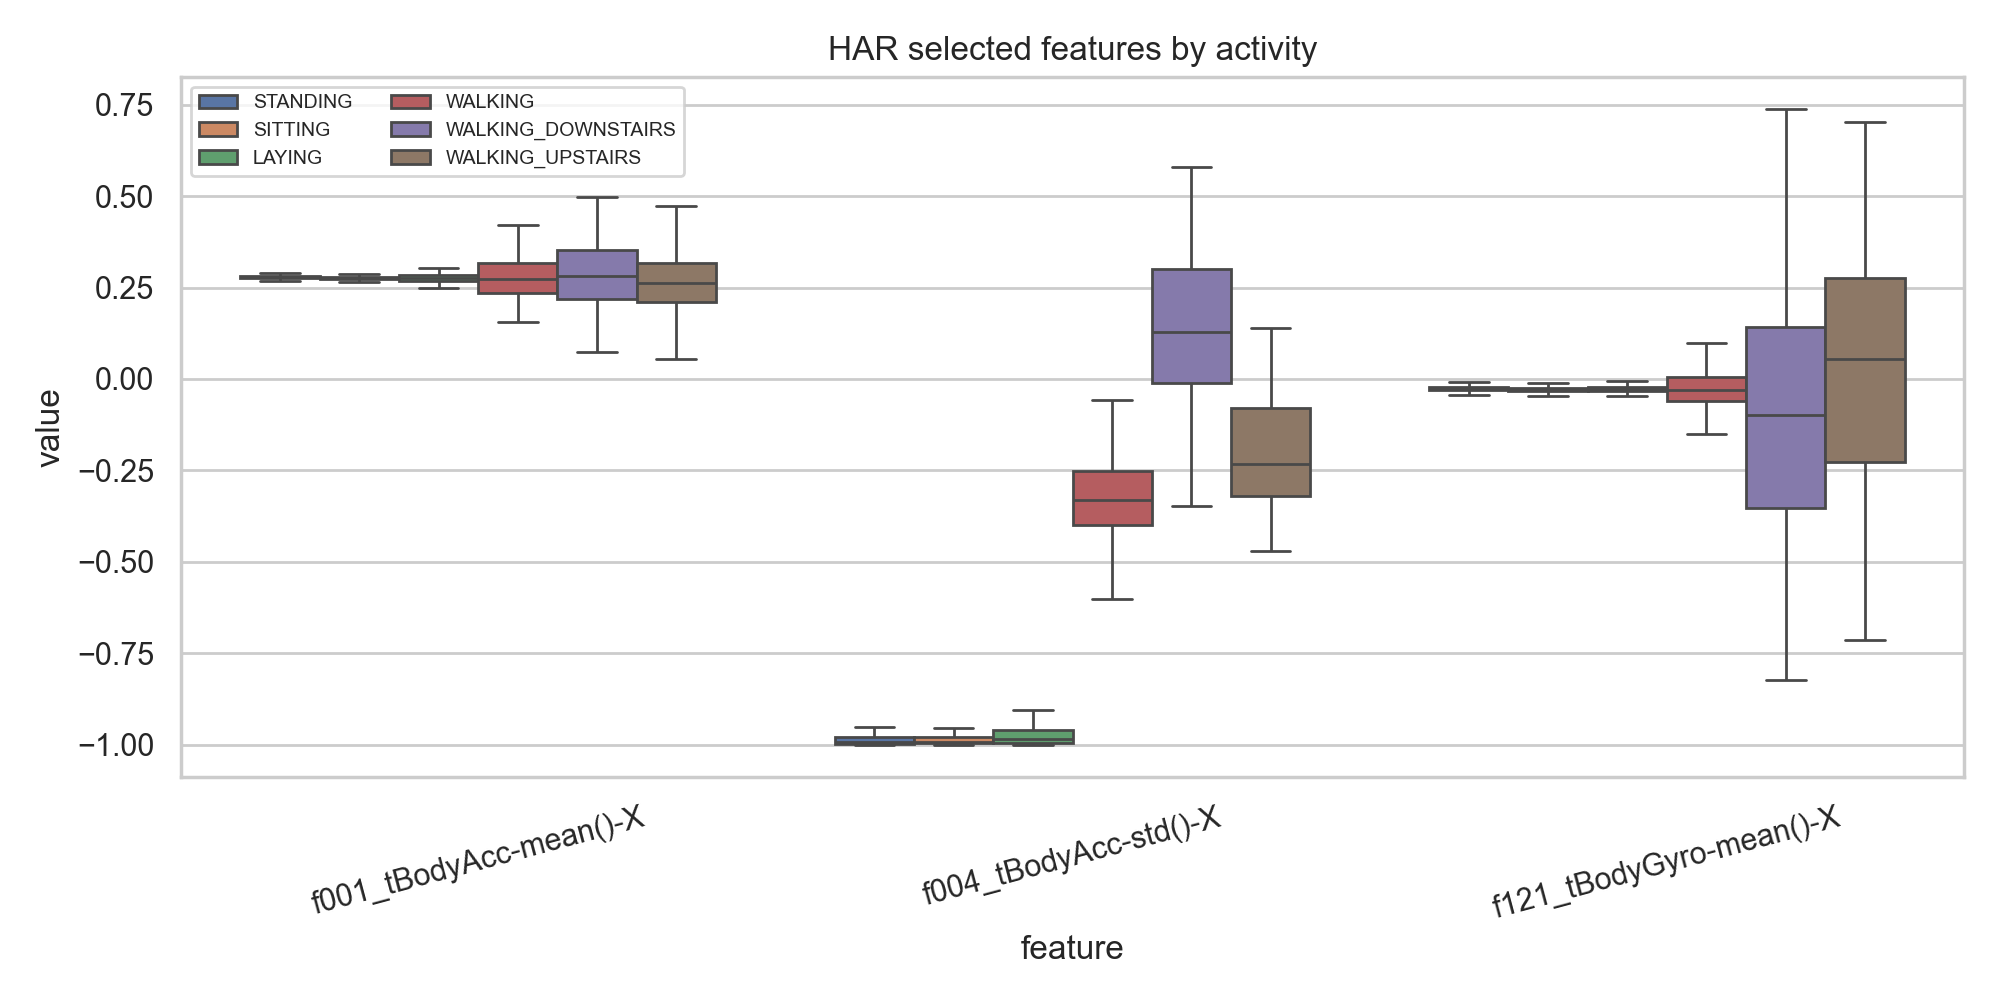
\includegraphics[width=\textwidth]{../outputs/figures/har_selected_feature_boxplot.png}
    \caption{Đặc trưng cảm biến theo activity}
\end{subfigure}
\caption[Minh họa HAR Smartphones]{Minh họa Human Activity Recognition Using Smartphones. Python source: \texttt{src/analyze\_har.py}; figure paths: \texttt{outputs/figures/har\_activity\_distribution.png}, \texttt{outputs/figures/har\_selected\_feature\_boxplot.png}.}
\label{fig:chapter2_har}
\end{figure}

\textbf{Kết quả ban đầu.} Hình \ref{fig:chapter2_har} cho thấy sáu hoạt động được ghi nhận tương đối đầy đủ, tạo điều kiện thuận lợi cho classification và clustering. Boxplot các đặc trưng gia tốc/gyro cho thấy một số hoạt động tĩnh và động có miền giá trị khác nhau, phù hợp với hướng dùng SVM, Random Forest hoặc CNN/LSTM trên tín hiệu raw.

\subsection{B3 - MHEALTH Dataset}

\textbf{Nguồn gốc và cấu trúc dữ liệu.} MHEALTH là bộ dữ liệu Mobile Health từ UCI, được lưu tại \path{datasets/MHEALTHDATASET/MHEALTHDATASET/}. Dữ liệu gồm 10 file subject log, tổng cộng 1,215,745 dòng, 23 features cảm biến và 1 cột activity label. Các cảm biến được đặt trên nhiều vị trí cơ thể, thu thập gia tốc, gyro, từ trường và tín hiệu liên quan sức khỏe.

\textbf{Trường dữ liệu và phân phối.} Mỗi dòng là một thời điểm trong log cảm biến, chưa phải một mẫu học máy độc lập theo nghĩa cửa sổ thời gian. Trong mẫu phân tích, nhãn NULL chiếm 282,379 dòng (70.59\%), lớn hơn nhiều so với các hoạt động thực như standing still 24,576 (6.14\%), sitting 21,568 (5.39\%), lying 18,496 (4.62\%), walking 16,960 (4.24\%), waist bends 13,684 (3.42\%) và climbing stairs 12,288 (3.07\%). Điều này cho thấy dữ liệu rất giàu về thời lượng ghi nhận nhưng mất cân bằng nghiêm trọng theo nhãn. Các trường \texttt{sensor\_01}--\texttt{sensor\_23} đại diện cho nhiều kênh đo; khi phân tích cần nhóm theo vị trí/cảm biến, chuẩn hóa scale, lọc nhãn NULL và chuyển log dài thành cửa sổ trượt có đặc trưng mean, variance, RMS, energy hoặc FFT.

\textbf{Tổng quan bài báo liên quan.} Banos và cộng sự xây dựng MHEALTH để đánh giá nhận dạng hoạt động và theo dõi sức khỏe bằng cảm biến đa vị trí trên cơ thể \cite{Banos2014MHEALTH}. Bài báo nhấn mạnh ưu điểm của dữ liệu đa kênh: cùng một hoạt động được quan sát từ nhiều vị trí cơ thể, giúp mô hình học được cả chuyển động cục bộ và toàn thân. Kết quả/ý nghĩa của nghiên cứu là cung cấp benchmark lớn cho activity recognition trong bối cảnh mobile health, nơi yêu cầu vừa nhận dạng hoạt động vừa hỗ trợ giám sát sức khỏe. Trong báo cáo này, phân phối NULL quá lớn cho thấy cần tiền xử lý mạnh hơn HAR: loại bỏ đoạn không hoạt động, cân bằng lớp và tạo cửa sổ trượt trước khi dùng SVM, Random Forest, CNN 1D hoặc LSTM.

\begin{table}[H]
\centering
\caption{So sánh hai bộ dữ liệu cảm biến nhóm B}
\label{tab:sensor_dataset_compare}
\small
\begin{tabular}{llll}
\toprule
Bộ dữ liệu & Số mẫu & Số đặc trưng & Điểm mạnh \\
\midrule
HAR & 10299 & 561 & Feature vector đã xử lý, nhãn hoạt động rõ \\
MHEALTH & 1215745 & 23 & Dữ liệu log dài, nhiều subject, cảm biến đa vị trí \\
\bottomrule
\end{tabular}
\end{table}

\begin{table}[H]
\centering
\caption{Thống kê mô tả các thuộc tính chính của MHEALTH}
\label{tab:mhealth_descriptive_stats}
\small
\begin{tabular}{lllll}
\toprule
Thuộc tính & Loại & Trung bình & Độ phân tán & Ghi chú \\
\midrule
sensor\_01 & Liên tục & -3.80 & std = 4.25 & Gia tốc/ngực \\
sensor\_02 & Liên tục & -9.44 & std = 3.30 & Gia tốc/ngực \\
sensor\_03 & Liên tục & 1.92 & std = 4.07 & Gia tốc/ngực \\
sensor\_10 & Liên tục & -0.34 & std = 0.57 & Kênh cảm biến khác \\
activity & Định tính & -- & NULL 70.59\% & Target mất cân bằng \\
\bottomrule
\end{tabular}
\end{table}

\begin{figure}[H]
\centering
\begin{subfigure}{0.92\textwidth}
    \centering
    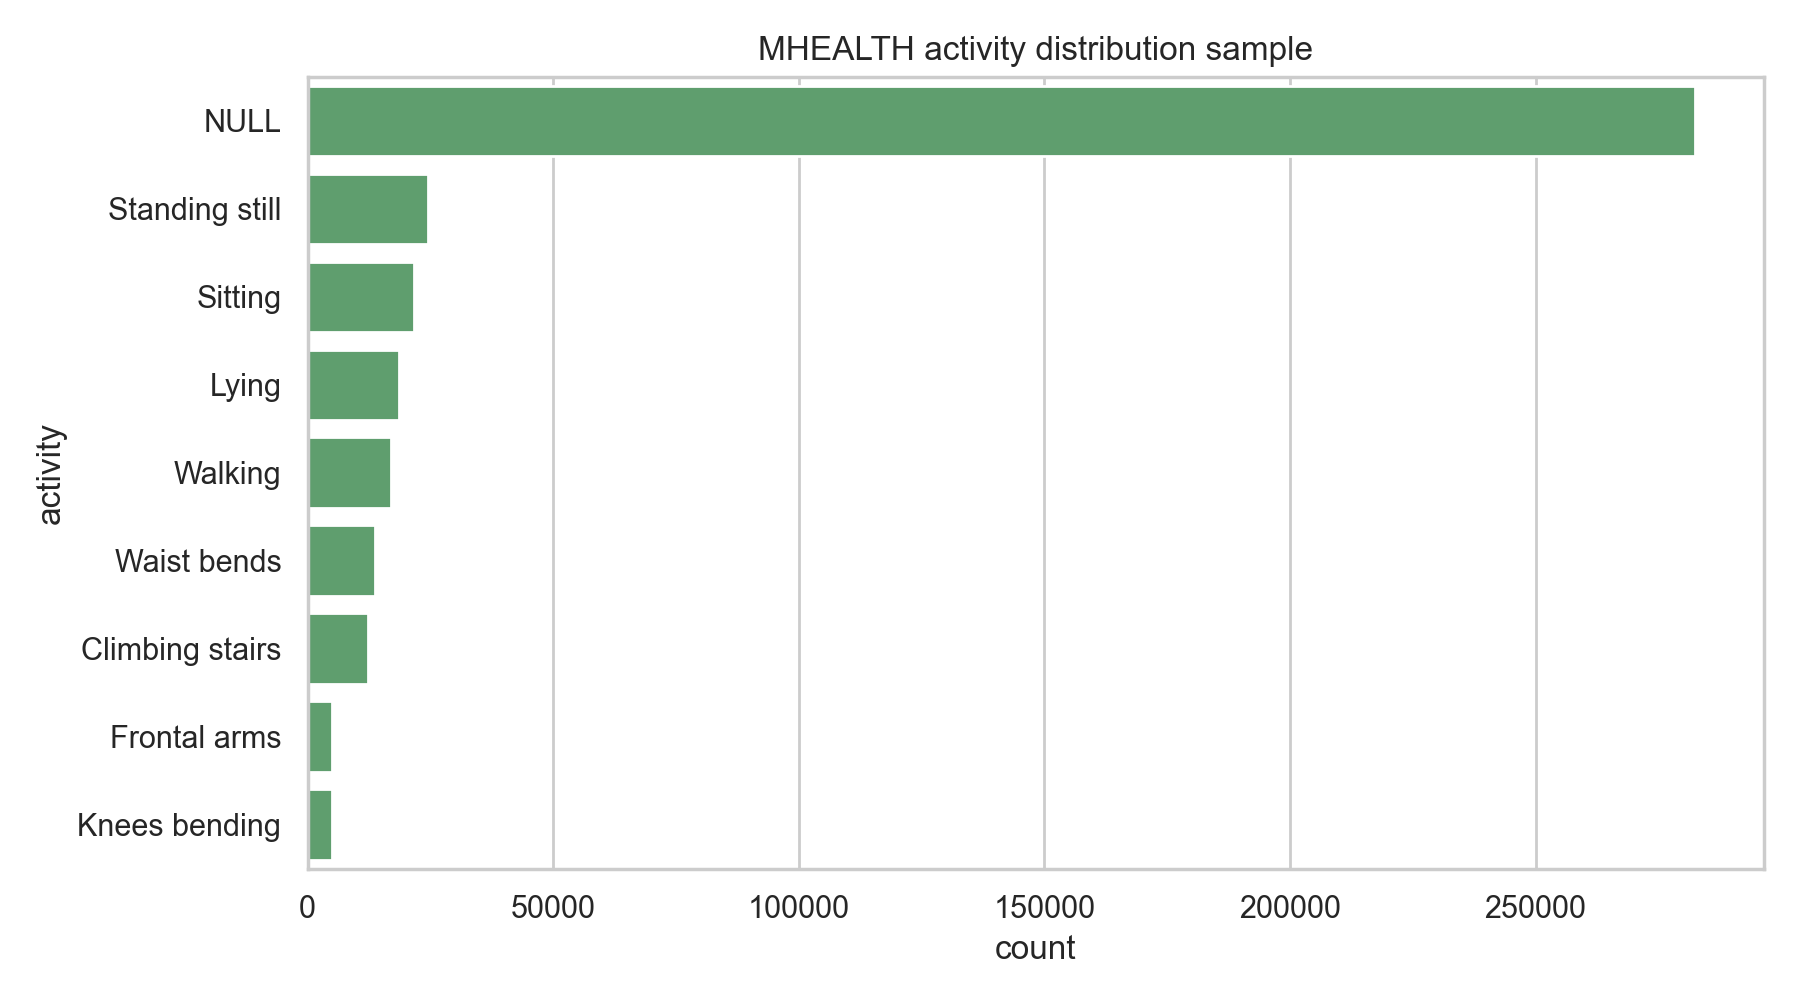
\includegraphics[width=\textwidth]{../outputs/figures/mhealth_activity_distribution.png}
    \caption{Phân phối activity trên mẫu}
\end{subfigure}

\vspace{0.4cm}

\begin{subfigure}{0.92\textwidth}
    \centering
    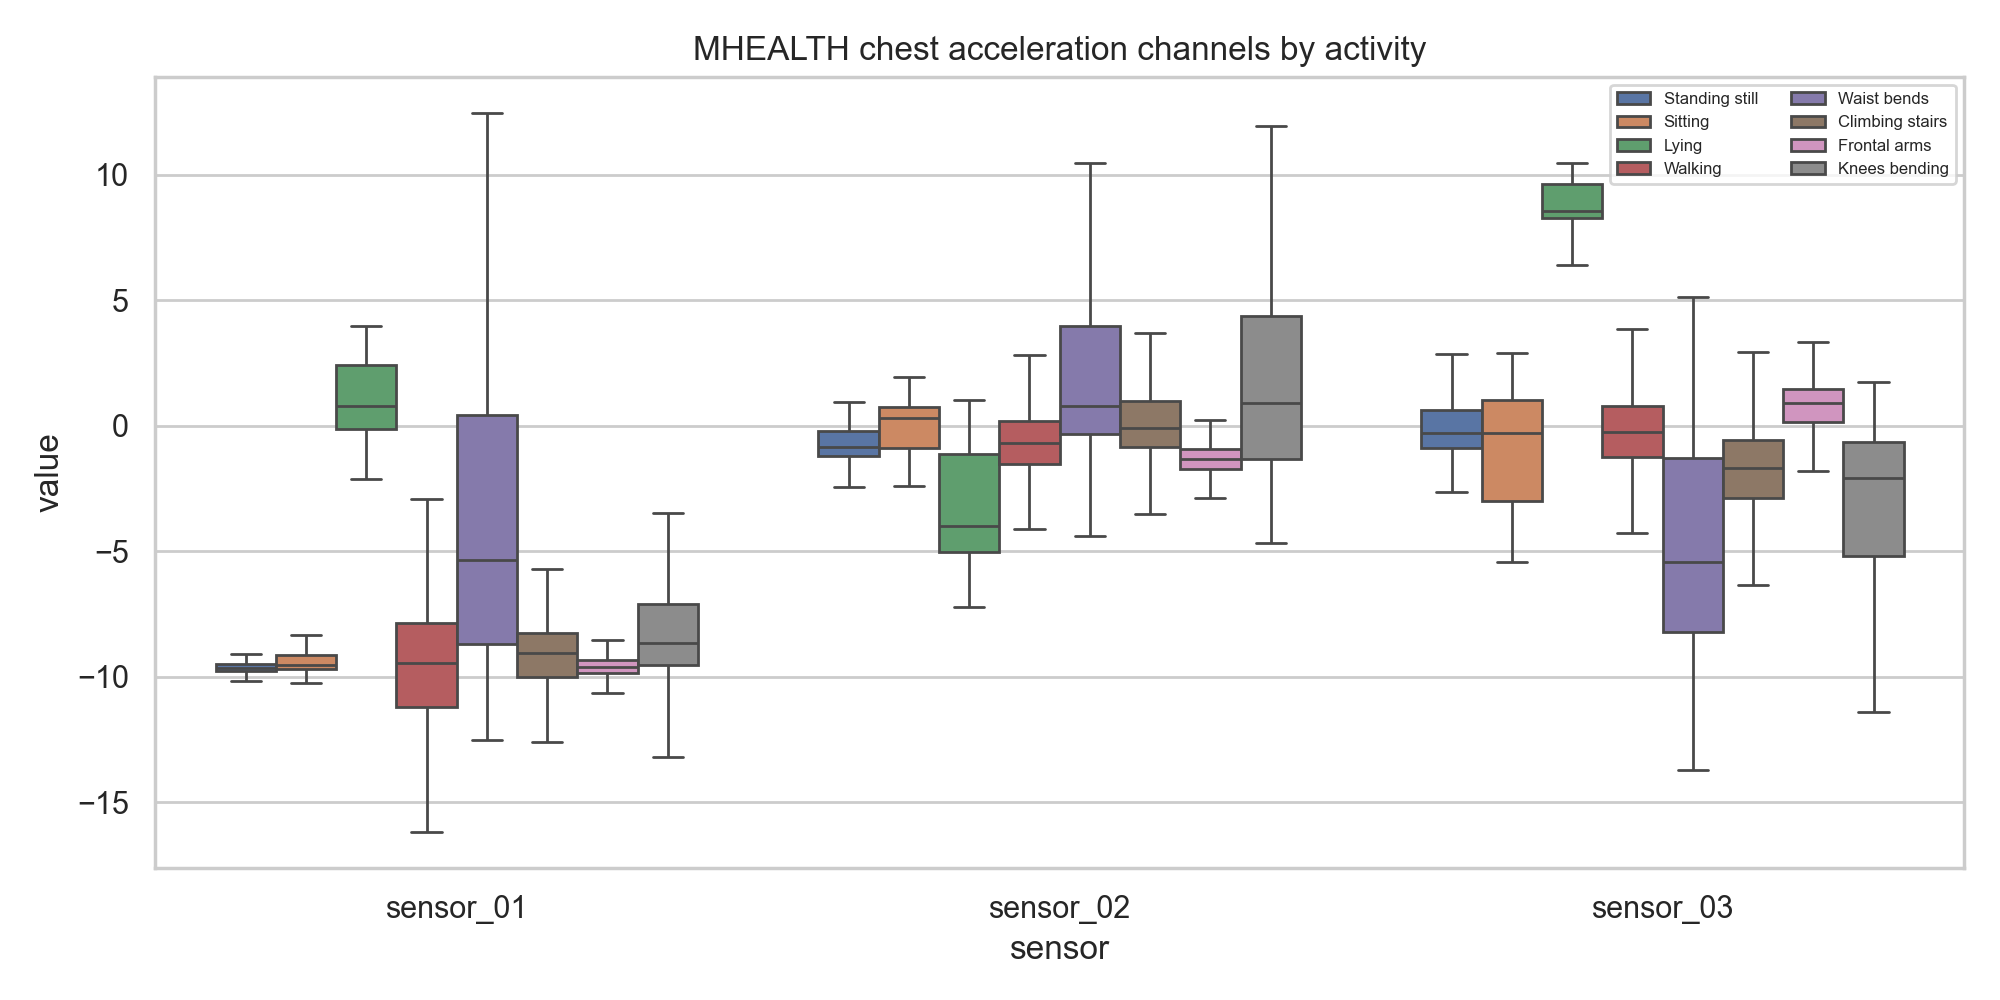
\includegraphics[width=\textwidth]{../outputs/figures/mhealth_sensor_boxplot.png}
    \caption{Kênh cảm biến theo activity}
\end{subfigure}
\caption[Minh họa MHEALTH]{Minh họa MHEALTH Dataset. Python source: \texttt{src/analyze\_mhealth.py}; figure paths: \texttt{outputs/figures/mhealth\_activity\_distribution.png}, \texttt{outputs/figures/mhealth\_sensor\_boxplot.png}.}
\label{fig:chapter2_mhealth}
\end{figure}

\textbf{Kết quả ban đầu.} Hình \ref{fig:chapter2_mhealth} cho thấy dữ liệu MHEALTH có nhiều nhãn hoạt động và log cảm biến lớn. Hoạt động null chiếm nhiều dòng trong mẫu, vì vậy khi huấn luyện cần lọc hoặc cân bằng nhãn. Các kênh gia tốc ngực có phân phối khác nhau theo hoạt động, xác nhận dữ liệu phù hợp cho nhận dạng hoạt động bằng đặc trưng cửa sổ trượt.

\section{Nhóm C: Dữ liệu đa phương tiện}

Nhóm C chọn hai dạng dữ liệu đa phương tiện: ảnh và văn bản. Với nhóm này, mô tả không chỉ gồm số dòng mà còn phải nêu định dạng file gốc và cách chuyển dữ liệu thô thành đặc trưng số để thống kê/học máy.

\begin{table}[H]
\centering
\caption{Thông tin file gốc và đặc trưng trích xuất của nhóm C}
\label{tab:group_c_file_format_summary}
\small
\begin{tabular}{p{0.18\textwidth}p{0.14\textwidth}p{0.16\textwidth}p{0.20\textwidth}p{0.20\textwidth}}
\toprule
Dataset & Loại media & Số lượng & Định dạng gốc & Đặc trưng trích xuất \\
\midrule
C1 HAM10000 & Ảnh & 10015 ảnh & JPG + metadata CSV & width, height, mean/std intensity, dx \\
C2 Reuters & Văn bản & 21578 tài liệu & 22 file SGML & word count, char count, topic, TF-IDF \\
\bottomrule
\end{tabular}
\end{table}

\begin{table}[H]
\centering
\caption{Phương pháp trích xuất đặc trưng cho dữ liệu đa phương tiện}
\label{tab:group_c_feature_extraction_methods}
\small
\begin{tabular}{p{0.16\textwidth}p{0.22\textwidth}p{0.24\textwidth}p{0.24\textwidth}}
\toprule
Dataset & Truyền thống & Học sâu & Nghiên cứu liên quan \\
\midrule
HAM10000 & Histogram màu, texture, shape, ABCD & CNN, transfer learning ResNet/EfficientNet & Tschandl et al.; Esteva et al. \\
Reuters & Bag-of-words, TF-IDF, n-gram, chọn đặc trưng & Embedding, CNN/RNN, Transformer & Lewis; Joachims; Sebastiani \\
\bottomrule
\end{tabular}
\end{table}

\subsection{C1 - HAM10000}

\textbf{Nguồn gốc và cấu trúc dữ liệu.} HAM10000 là bộ dữ liệu ảnh da liễu từ Kaggle, được chuẩn bị bằng \texttt{kagglehub}. Metadata được lưu tại \path{datasets/ham10000/}; ảnh gốc nằm trong KaggleHub cache và đường dẫn được ghi tại \path{datasets/ham10000/source_path.txt}. Bộ dữ liệu có 10,015 ảnh, 7 lớp chẩn đoán, 7 cột metadata và 7,470 lesion duy nhất.

\textbf{Trường dữ liệu và phân phối.} Metadata gồm \texttt{lesion\_id}, \texttt{image\_id}, \texttt{dx}, \texttt{dx\_type}, \texttt{age}, \texttt{sex} và \texttt{localization}. Target \texttt{dx} mất cân bằng rất mạnh: \texttt{nv} có 6,705 ảnh (66.95\%), \texttt{mel} 1,113 (11.11\%), \texttt{bkl} 1,099 (10.97\%), \texttt{bcc} 514 (5.13\%), \texttt{akiec} 327 (3.27\%), \texttt{vasc} 142 (1.42\%) và \texttt{df} 115 (1.15\%). Ngoài nhãn bệnh, tuổi, giới tính, vị trí tổn thương và kiểu xác nhận chẩn đoán là các biến quan trọng để phân tích bias dữ liệu. Trong báo cáo, ảnh được số hóa trên mẫu 1,000 ảnh bằng width, height, mode màu, mean intensity và standard deviation intensity; đây là đặc trưng mô tả ban đầu, chưa đủ thay thế đặc trưng màu, hình dạng, texture hoặc embedding CNN.

\textbf{Tổng quan bài báo liên quan.} Tschandl, Rosendahl và Kittler công bố HAM10000 như một tập ảnh da liễu lớn nhằm hỗ trợ huấn luyện hệ thống phân loại tổn thương sắc tố \cite{Tschandl2018HAM10000}. Bài báo tóm tắt quá trình thu thập ảnh, chuẩn hóa metadata và xây dựng nhãn đa lớp, đồng thời nhấn mạnh thách thức mất cân bằng lớp. Esteva và cộng sự cho thấy CNN có thể đạt hiệu quả ở mức chuyên gia da liễu trong phân loại ung thư da, qua đó chứng minh hướng transfer learning rất phù hợp với ảnh y khoa \cite{Esteva2017Dermatologist}. Kết quả/ý nghĩa của hai hướng nghiên cứu là: dữ liệu ảnh cần mô hình khai thác không gian-màu sắc tốt hơn đặc trưng thống kê đơn giản, nhưng đánh giá phải chú ý lớp hiếm. Vì vậy báo cáo dùng macro-F1, confusion matrix, augmentation và class weighting như hướng mở rộng hợp lý.

\begin{table}[H]
\centering
\caption{Phân phối lớp chẩn đoán trong HAM10000}
\label{tab:ham_class_distribution}
\small
\begin{tabular}{lrr}
\toprule
Lớp & Số ảnh & Tỷ lệ \\
\midrule
nv & 6705 & 66.95\% \\
mel & 1113 & 11.11\% \\
bkl & 1099 & 10.97\% \\
bcc & 514 & 5.13\% \\
akiec & 327 & 3.27\% \\
vasc & 142 & 1.42\% \\
df & 115 & 1.15\% \\
\bottomrule
\end{tabular}
\end{table}

\begin{table}[H]
\centering
\caption{Thống kê mô tả các thuộc tính chính của HAM10000}
\label{tab:ham_descriptive_stats}
\small
\begin{tabular}{lllll}
\toprule
Thuộc tính & Loại & Trung bình & Độ phân tán & Ghi chú \\
\midrule
age & Liên tục & 51.86 & std = 16.97 & Tuổi bệnh nhân \\
width & Rời rạc & 600.00 & std = 0.00 & Mẫu ảnh đã chuẩn hóa \\
height & Rời rạc & 450.00 & std = 0.00 & Mẫu ảnh đã chuẩn hóa \\
mean\_intensity & Liên tục & 157.47 & std = 18.65 & Độ sáng trung bình \\
std\_intensity & Liên tục & 46.11 & std = 8.52 & Độ phân tán pixel \\
dx & Định tính & -- & nv 66.95\% & Target mất cân bằng \\
\bottomrule
\end{tabular}
\end{table}

\begin{figure}[H]
\centering
\begin{subfigure}{0.92\textwidth}
    \centering
    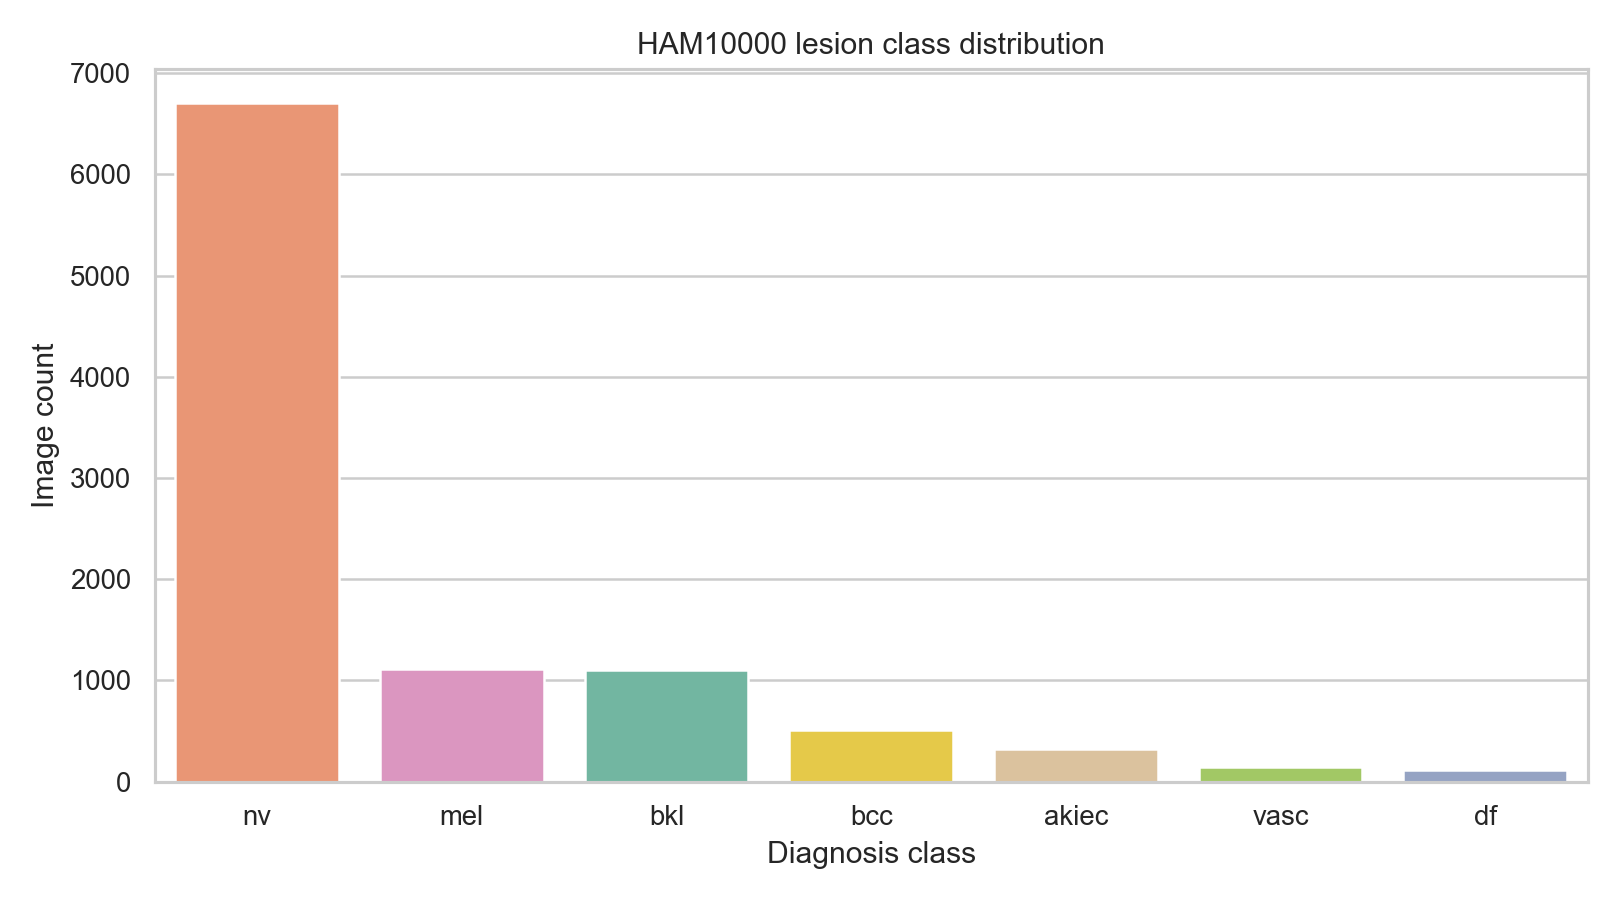
\includegraphics[width=\textwidth]{../outputs/figures/ham10000_class_distribution.png}
    \caption{Phân phối lớp}
\end{subfigure}

\vspace{0.4cm}

\begin{subfigure}{0.92\textwidth}
    \centering
    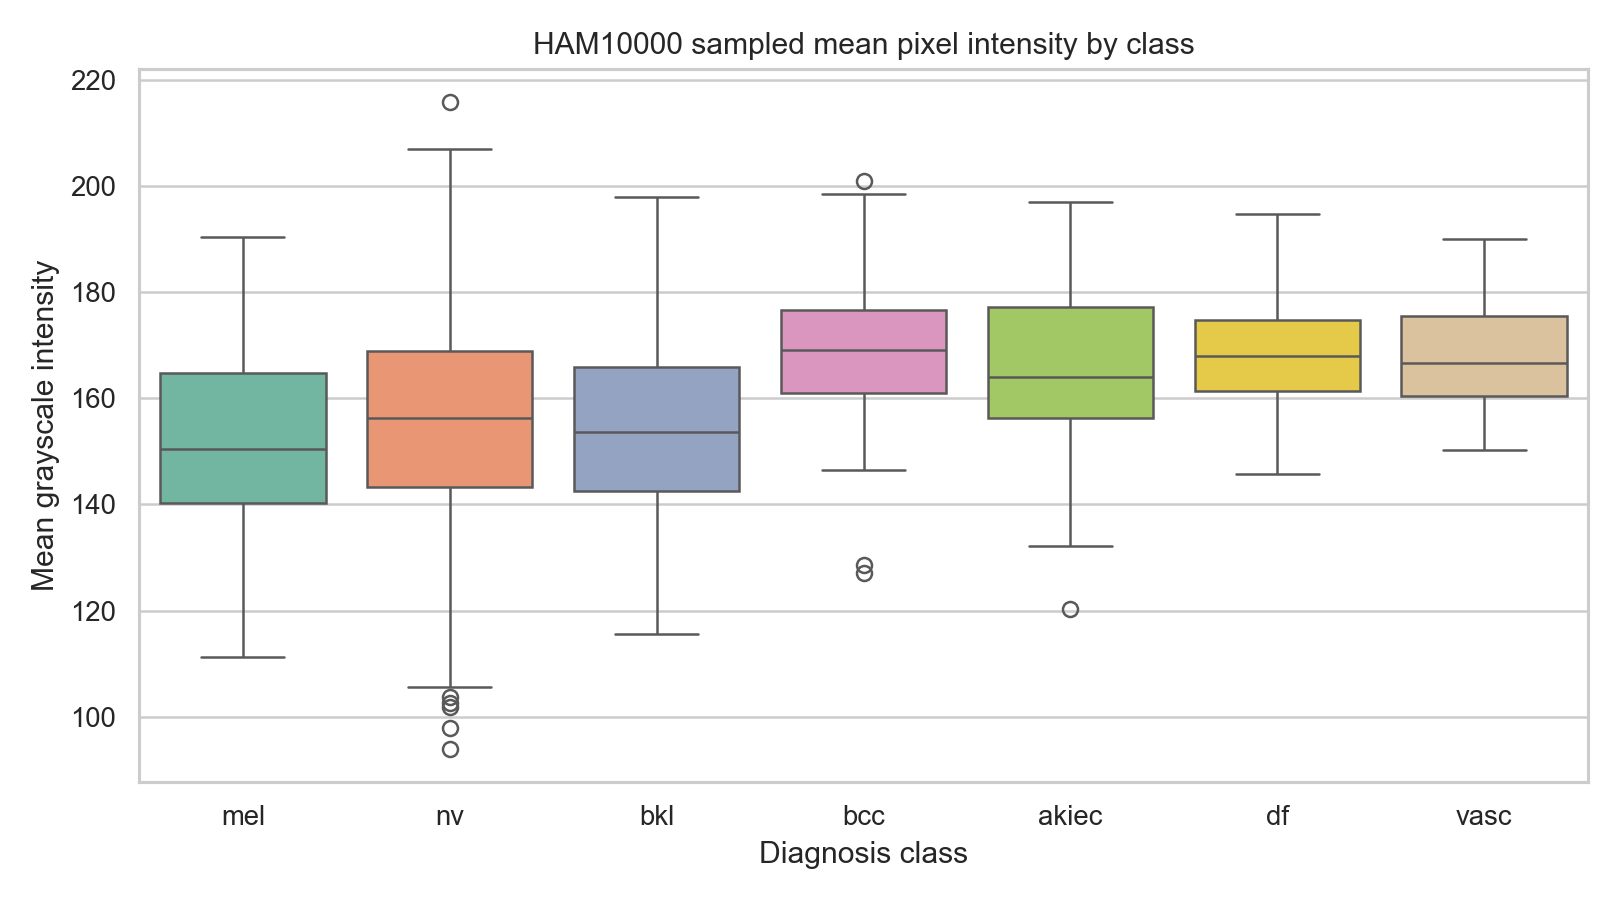
\includegraphics[width=\textwidth]{../outputs/figures/ham10000_mean_intensity_boxplot.png}
    \caption{Độ sáng trung bình theo lớp}
\end{subfigure}
\caption[Minh họa phân tích dữ liệu ảnh HAM10000 sau khi số hóa]{Minh họa phân tích dữ liệu ảnh HAM10000 sau khi số hóa. Python source: \texttt{src/analyze\_ham10000.py}; figure paths: \texttt{outputs/figures/ham10000\_class\_distribution.png}, \texttt{outputs/figures/ham10000\_mean\_intensity\_boxplot.png}.}
\label{fig:chapter2_ham10000}
\end{figure}

\textbf{Lý do chọn biểu đồ.} Bar chart phân phối lớp được chọn để kiểm tra mất cân bằng nhãn; boxplot độ sáng trung bình được chọn để xem đặc trưng ảnh sau số hóa có khác nhau giữa các lớp hay không.

\textbf{Nhận xét.} Bảng \ref{tab:ham_class_distribution} và Hình \ref{fig:chapter2_ham10000} chỉ ra vấn đề mất cân bằng lớp rất rõ. Lớp \texttt{nv} chiếm gần 67\%, trong khi \texttt{df} chỉ khoảng 1.15\%. Nếu mô hình chỉ học cách dự đoán lớp đa số, accuracy có thể cao nhưng khả năng phát hiện các lớp hiếm sẽ kém.

\textbf{Kết quả ban đầu.} Phân tích metadata và mẫu đặc trưng ảnh cho thấy tuổi bệnh nhân, vị trí tổn thương và độ sáng trung bình đều có thể dùng như biến mô tả bổ sung. Tuy nhiên, riêng đặc trưng intensity chưa đủ thay thế ảnh gốc; thí nghiệm chính nên dùng thêm đặc trưng màu/texture hoặc transfer learning để khai thác thông tin không gian của lesion.

\subsection{C2 - Reuters-21578 Text Categorization}

\textbf{Nguồn gốc và cấu trúc dữ liệu.} Reuters-21578 là bộ dữ liệu text categorization từ UCI/KDD Archive, được giải nén tại \path{datasets/reuters21578/}. Bộ dữ liệu có 21,578 tài liệu trong 22 file SGML và các file từ điển category liên quan. Mỗi tài liệu có thể chứa tiêu đề, nội dung, topic, place, people, organization và các metadata khác.

\textbf{Trường dữ liệu và phân phối.} Để phân tích thống kê, SGML được parse thành bảng đặc trưng gồm mã tài liệu, topic chính, số từ và số ký tự. Top topic có phân phối dài đuôi: \texttt{earn} có 3,972 tài liệu, \texttt{acq} 2,423, \texttt{money-fx} 682, \texttt{crude} 543, \texttt{grain} 537, \texttt{trade} 473, \texttt{interest} 339, \texttt{ship} 209, \texttt{money-supply} 177 và \texttt{sugar} 154. Độ dài văn bản biến thiên mạnh, nên cần chuẩn hóa text, loại stopword, xử lý token hiếm và dùng TF-IDF để giảm ảnh hưởng của văn bản quá dài. Vì nhiều topic nhỏ có ít mẫu, accuracy dễ bị chi phối bởi lớp lớn; macro-F1 và per-class recall phù hợp hơn khi đánh giá.

\textbf{Tổng quan bài báo liên quan.} Lewis mô tả và chuẩn hóa Reuters-21578 như benchmark kinh điển cho text categorization, giúp cộng đồng có một bộ tin tức gán nhãn để so sánh thuật toán phân loại văn bản \cite{Lewis1997Reuters}. Joachims dùng Reuters để đánh giá SVM cho text classification và chỉ ra rằng SVM phù hợp với vector văn bản thưa, nhiều chiều vì có khả năng tìm siêu phẳng phân tách tốt trong không gian TF-IDF \cite{Joachims1998TextSVM}. Sebastiani tổng quan các kỹ thuật machine learning cho text categorization, trong đó Reuters là bộ dữ liệu đối sánh quan trọng để so sánh Naive Bayes, k-NN, SVM và các phương pháp chọn đặc trưng \cite{Sebastiani2002TextCategorization}. Kết quả/ý nghĩa chung là xác lập pipeline cổ điển cho text mining: parse văn bản, vector hóa bằng bag-of-words/TF-IDF, chọn đặc trưng và dùng mô hình tuyến tính; báo cáo hiện tại đi theo pipeline này ở mức chuẩn bị đặc trưng ban đầu.

\begin{table}[H]
\centering
\caption{Kế hoạch số hóa dữ liệu text Reuters-21578}
\label{tab:reuters_feature_plan}
\small
\begin{tabular}{lll}
\toprule
Nhóm đặc trưng & Ví dụ & Mục đích \\
\midrule
Độ dài văn bản & số từ, số ký tự, số câu & Thống kê mô tả và outlier \\
Từ vựng & tần suất từ, stop word ratio & Mô tả phong cách nội dung \\
Vector hóa & TF-IDF unigram/bigram & Input cho classification \\
Nhãn chủ đề & topics, places, orgs & Target và phân tích tần suất \\
\bottomrule
\end{tabular}
\end{table}

\begin{table}[H]
\centering
\caption{Thống kê mô tả các thuộc tính chính của Reuters-21578}
\label{tab:reuters_descriptive_stats}
\small
\begin{tabular}{lllll}
\toprule
Thuộc tính & Loại & Trung bình & Độ phân tán & Ghi chú \\
\midrule
word\_count & Rời rạc & 72.31 & std = 145.78 & Độ dài văn bản \\
char\_count & Rời rạc & 439.64 & std = 873.51 & Số ký tự \\
primary\_topic & Định tính & -- & earn 3972 & Target dài đuôi \\
topics & Multi-label & -- & nhiều nhãn & Chủ đề văn bản \\
newid & Định danh & -- & -- & Mã tài liệu \\
\bottomrule
\end{tabular}
\end{table}

\begin{figure}[H]
\centering
\begin{subfigure}{0.92\textwidth}
    \centering
    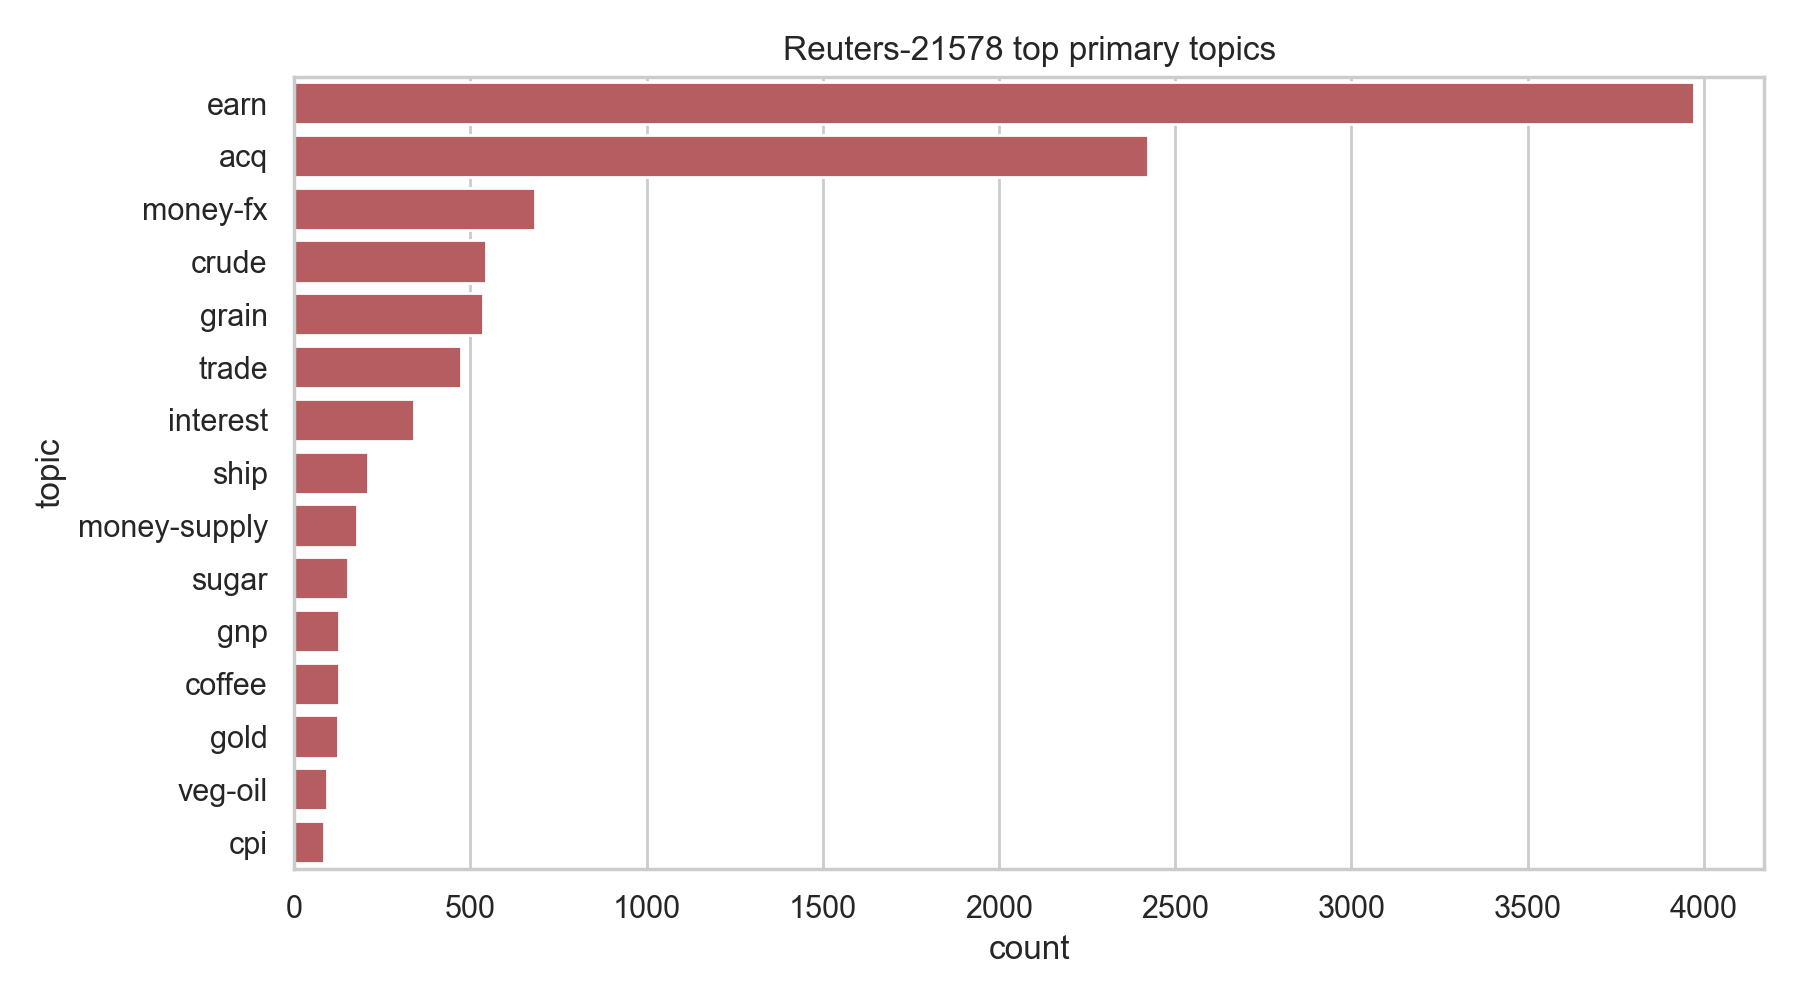
\includegraphics[width=\textwidth]{../outputs/figures/reuters_top_topics.png}
    \caption{Top topic chính}
\end{subfigure}

\vspace{0.4cm}

\begin{subfigure}{0.92\textwidth}
    \centering
    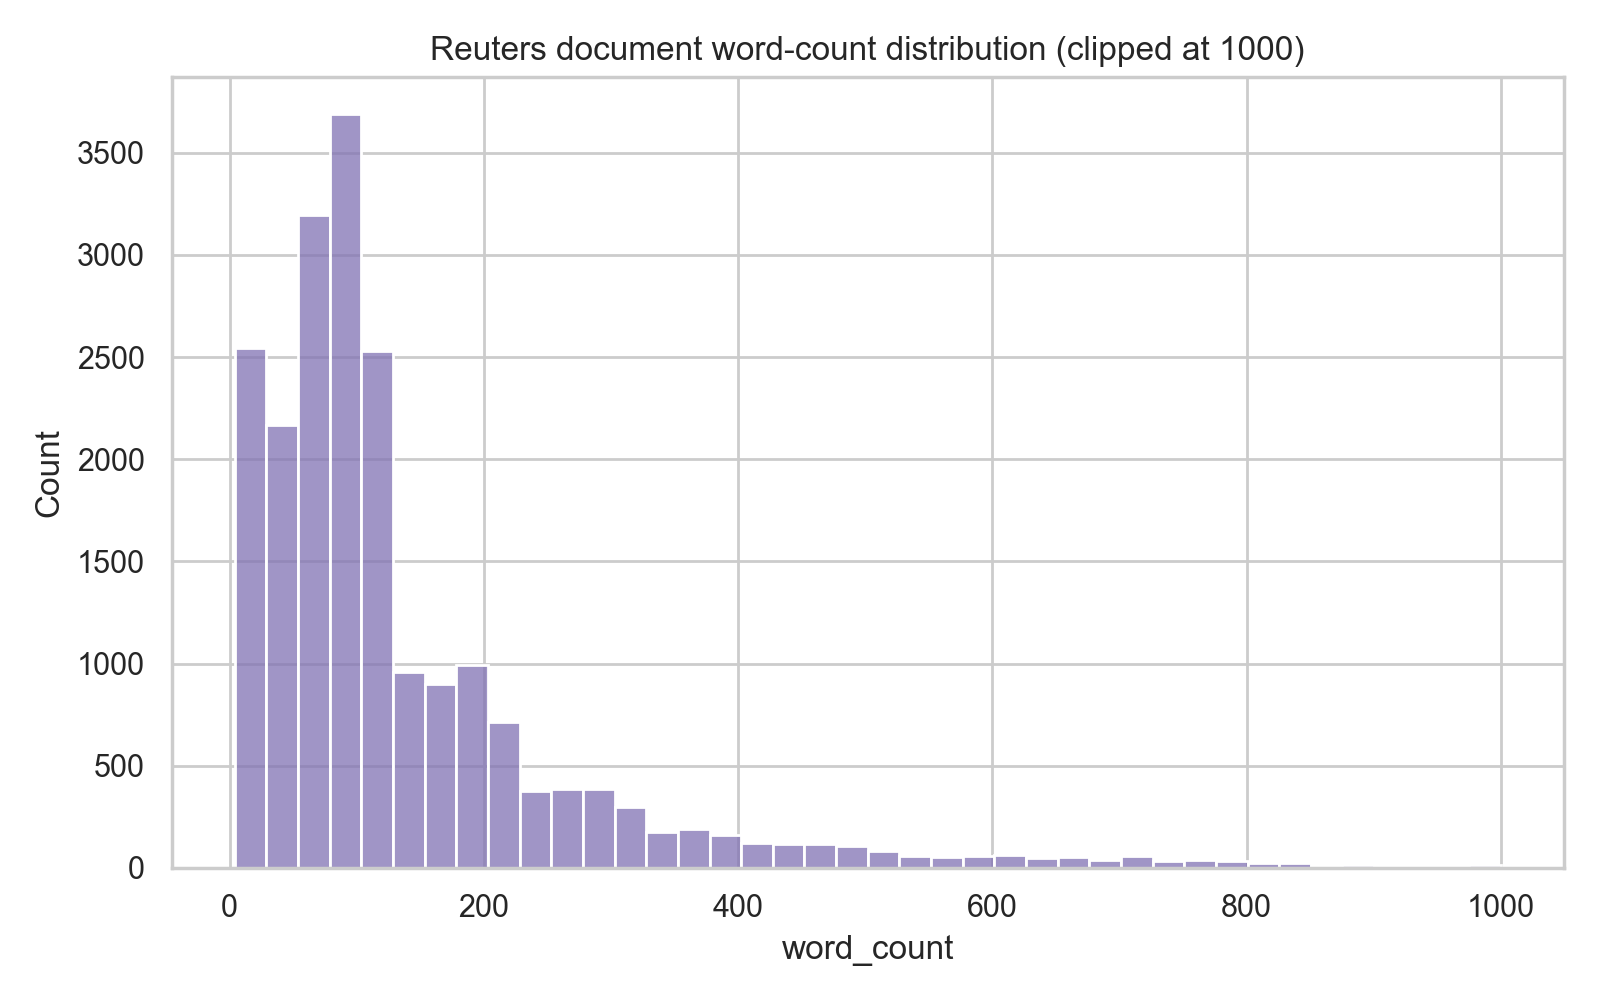
\includegraphics[width=\textwidth]{../outputs/figures/reuters_word_count_histogram.png}
    \caption{Phân phối số từ}
\end{subfigure}
\caption[Minh họa Reuters-21578]{Minh họa Reuters-21578 sau khi parse SGML. Python source: \texttt{src/analyze\_reuters.py}; figure paths: \texttt{outputs/figures/reuters\_top\_topics.png}, \texttt{outputs/figures/reuters\_word\_count\_histogram.png}.}
\label{fig:chapter2_reuters}
\end{figure}

\textbf{Kết quả ban đầu.} Script parse SGML tạo bảng đặc trưng văn bản gồm topic chính, số từ và số ký tự cho từng tài liệu. Hình \ref{fig:chapter2_reuters} cho thấy topic có phân phối lệch và độ dài văn bản biến thiên mạnh; vì vậy mô hình text classification cần TF-IDF, chuẩn hóa văn bản và đánh giá macro-F1 thay vì chỉ accuracy.

\begin{table}[H]
\centering
\caption{Đối sánh nghiên cứu liên quan và baseline dùng cho Chương 4}
\label{tab:chapter2_research_benchmark}
\small
\begin{tabular}{p{0.18\textwidth}p{0.22\textwidth}p{0.26\textwidth}p{0.22\textwidth}}
\toprule
Dataset & Nghiên cứu & Kỹ thuật/thuật toán & Kết quả/ý nghĩa đối sánh \\
\midrule
Heart Disease & Detrano; Aha; Gennari & Mô hình xác suất, instance-based learning, CLASSIT & Benchmark lâm sàng; baseline RF của báo cáo đạt Acc 0.902, F1 0.897 \\
CDC Diabetes & BRFSS; Smith et al. & Phân tích yếu tố nguy cơ, LR/RF/SVM & Dữ liệu khảo sát mất cân bằng; SVM RBF mẫu đạt Acc 0.744, F1 0.761 \\
Breast Cancer & Street; Mangasarian & Trích đặc trưng FNA, hyperplane/SVM & Đặc trưng hình học phân tách mạnh; SVM RBF đạt Acc 0.982, F1 0.976 \\
Appliances & Candanedo et al. & RF, regression, feature thời gian & Forecasting cần lag/rolling; LR ban đầu RMSE 89.40, R2 0.036 \\
HAR/MHEALTH & Anguita; Banos & SVM, windowing, sensor features & Activity recognition cần cửa sổ tín hiệu và chuẩn hóa kênh \\
HAM10000/Reuters & Tschandl, Esteva; Lewis, Joachims & CNN/transfer learning; TF-IDF/SVM & Multimedia cần trích đặc trưng; đánh giá macro-F1 do mất cân bằng \\
\bottomrule
\end{tabular}
\end{table}

\begin{table}[H]
\centering
\caption{Baseline học máy nhóm A dùng làm mốc cho Chương 4}
\label{tab:chapter2_ml_preview}
\small
\begin{tabular}{llrrr}
\toprule
Dataset & Model & Accuracy & Recall & F1 \\
\midrule
Heart Disease & Logistic Regression & 0.869 & 0.929 & 0.867 \\
Heart Disease & Random Forest & 0.902 & 0.929 & 0.897 \\
Heart Disease & SVM RBF & 0.885 & 0.964 & 0.885 \\
CDC Diabetes & Logistic Regression & 0.744 & 0.775 & 0.752 \\
CDC Diabetes & Random Forest & 0.724 & 0.787 & 0.740 \\
CDC Diabetes & SVM RBF & 0.744 & 0.814 & 0.761 \\
Breast Cancer & Logistic Regression & 0.974 & 0.952 & 0.964 \\
Breast Cancer & Random Forest & 0.974 & 0.929 & 0.963 \\
Breast Cancer & SVM RBF & 0.982 & 0.976 & 0.976 \\
\bottomrule
\end{tabular}
\end{table}

Bảng \ref{tab:chapter2_research_benchmark} và Bảng \ref{tab:chapter2_ml_preview} là cầu nối giữa phần mô tả dữ liệu ở Chương 2 và thực nghiệm ở Chương 4. Các kết quả trong báo cáo không thay thế kết quả công bố của bài báo gốc, nhưng cung cấp mốc nội bộ để so sánh mô hình trên cùng pipeline tiền xử lý.


\section{Đánh giá chất lượng dữ liệu và rủi ro phân tích}

Mỗi nhóm dữ liệu có rủi ro phân tích khác nhau. Dữ liệu dạng bảng thường gặp missing value, outlier và mất cân bằng target. Dữ liệu chuỗi thời gian có rủi ro rò rỉ tương lai nếu chia train/test ngẫu nhiên. Dữ liệu đa phương tiện có rủi ro lớn hơn vì phải chuyển đổi file ảnh hoặc văn bản thô thành đặc trưng định lượng trước khi thống kê.

\begin{table}[H]
\centering
\caption{Rủi ro chất lượng dữ liệu và hướng xử lý}
\label{tab:chapter2_data_quality_risk}
\small
\begin{tabular}{p{0.20\textwidth}p{0.32\textwidth}p{0.34\textwidth}}
\toprule
Nhóm dữ liệu & Rủi ro chính & Hướng xử lý trong báo cáo \\
\midrule
Nhóm A & Missing value, outlier, target mất cân bằng & Điền khuyết, IQR, chuẩn hóa, confusion matrix \\
Nhóm B & Rò rỉ dữ liệu tương lai, seasonality, scale khác nhau & Tách theo thời gian, rolling/lag, log-transform \\
Nhóm C ảnh & Mất cân bằng lớp, ảnh khác kích thước/độ sáng & Trích xuất width, height, intensity, phân tích theo lớp \\
Nhóm C text & Văn bản dài/ngắn bất thường, nhiều topic & Word count, TF-IDF, bảng tần suất topic \\
\bottomrule
\end{tabular}
\end{table}

Bảng \ref{tab:chapter2_data_quality_risk} là cơ sở để liên kết Chương 2 với Chương 3. Sau khi mô tả nguồn dữ liệu, báo cáo cần chứng minh dữ liệu đủ tốt để phân tích, hoặc chỉ rõ biến nào cần làm sạch. Ví dụ, Heart Disease có missing value ở \texttt{ca} và \texttt{thal}; Appliances Energy không nên chia dữ liệu ngẫu nhiên; HAM10000 mất cân bằng lớp rất rõ; Reuters-21578 cần bước parse SGML và chuẩn hóa văn bản trước khi tạo đặc trưng.

\section{Liên hệ giữa nguồn dữ liệu và yêu cầu bài toán}

Yêu cầu bài tập gồm ba khối: thu thập dữ liệu, phân tích thống kê/trực quan hóa và học máy. Do đó, phần mô tả dữ liệu phải cho thấy mỗi dataset đóng góp gì cho từng yêu cầu. Nếu một dataset chỉ được mô tả nguồn gốc mà không được dùng để tính toán hoặc vẽ biểu đồ, báo cáo sẽ thiếu bằng chứng thực nghiệm.

\begin{table}[H]
\centering
\caption{Liên hệ dataset với các yêu cầu của đề bài}
\label{tab:chapter2_requirement_mapping}
\small
\begin{tabular}{p{0.22\textwidth}p{0.20\textwidth}p{0.26\textwidth}p{0.20\textwidth}}
\toprule
Dataset & Yêu cầu 1 & Yêu cầu 2 & Yêu cầu 3 \\
\midrule
Heart Disease & Dữ liệu bảng & Thống kê, histogram, boxplot, scatter & Classification \\
CDC Diabetes & Dữ liệu bảng lớn & Tần suất biến sức khỏe, BMI & Classification \\
Breast Cancer & Dữ liệu bảng y sinh & Histogram, heatmap, boxplot & Classification \\
Appliances Energy & Chuỗi thời gian & Line chart, log-transform & Regression \\
HAR & Chuỗi/cảm biến & Phân phối activity, cảm biến & Clustering/classification \\
MHEALTH & Chuỗi/cảm biến lớn & Thống kê tín hiệu & Clustering/classification \\
HAM10000 & Ảnh & Số hóa ảnh, class distribution & Image classification \\
Reuters-21578 & Text & Word count, topic frequency & Text classification \\
\bottomrule
\end{tabular}
\end{table}

Bảng \ref{tab:chapter2_requirement_mapping} giúp người đọc thấy rõ dữ liệu không bị chọn rời rạc. Mỗi bộ dữ liệu là một mắt xích của chuỗi yêu cầu: từ nguồn dữ liệu, sang thống kê/trực quan hóa, rồi sang mô hình học máy.

\section{Các dữ liệu và nội dung cần bổ sung tiếp}

Dù Chương 2 đã mô tả đủ 8 bộ dữ liệu, bài báo liên quan, phân phối chính và kết quả ban đầu, báo cáo vẫn cần các bước hoàn thiện sau để phục vụ bản final:

\begin{itemize}
    \item Chuyển bảng mô tả biến đầy đủ của từng dataset sang phụ lục để tránh làm Chương 2 quá dài.
    \item Mở rộng thí nghiệm clustering trên cả dữ liệu bảng, chuỗi thời gian/cảm biến và multimedia.
    \item Bổ sung bảng tổng hợp đường dẫn raw data, cleaned data, source code, log và output cho từng hình/bảng.
    \item Chuẩn hóa toàn bộ trích dẫn theo một kiểu thống nhất trước khi nộp bản final.
\end{itemize}

Các mục trên là phần hoàn thiện phụ lục và thực nghiệm, không phải thiếu sót cốt lõi của Chương 2. Nội dung chính của chương hiện đã liên kết được nguồn dữ liệu, trường dữ liệu, phân phối, bài báo liên quan và kết quả phân tích ban đầu.

\section{Đường dẫn minh chứng và tái sử dụng}

Tất cả dữ liệu, script và kết quả được lưu lại để phục vụ phụ lục. Bảng minh chứng tổng hợp được sinh bằng \path{src/build_evidence_index.py} và lưu tại \path{outputs/tables/evidence_index.csv}. Cách tổ chức này giúp mỗi bảng/hình trong báo cáo đều có thể truy vết nguồn dữ liệu, script xử lý và file kết quả tương ứng.
